\documentclass[specialist,
               substylefile = spbu.rtx,
               subf,href,colorlinks=true, 12pt]{disser}
\usepackage[breakable]{tcolorbox}
\usepackage[a4paper,left=3cm, right=1.5cm, top=2cm, bottom=2cm, headsep=1cm, footskip=1cm]{geometry}
\usepackage[utf8]{inputenc}
\usepackage[T2A]{fontenc}
\usepackage{graphicx}
\usepackage[english,russian]{babel}
\usepackage{amsfonts}
\usepackage{amsmath}
\usepackage{bm}
\usepackage{float}
\usepackage{amsthm}
%\usepackage{parskip} % Stop auto-indenting (to mimic markdown behaviour)
\usepackage[ruled,vlined]{algorithm2e}
\usepackage{physics}
\newtheorem{statement}{Утверждение}
\newtheorem{theorem}{Теорема}
\newtheorem*{statement*}{Утверждение}
\newtheorem*{notice*}{Замечание}
\newtheorem{lemma}{Лемма}  
\newtheorem*{def*}{Определение}  

\DeclareMathOperator{\rk}{rk}
\DeclareMathOperator{\med}{med}
\DeclareMathOperator{\diag}{diag}
\DeclareMathOperator{\sign}{sign}
%\DeclareMathOperator{\tr}{tr}
\newcommand{\tX}[1]{\mathsf{#1}}
%\newcommand{\norm}[1]{\left\lVert#1\right\rVert}
\DeclareMathOperator*{\argminB}{argmin}

\geometry{verbose,tmargin=1in,bmargin=1in,lmargin=1in,rmargin=1in}

\DeclareMathOperator*{\argmin}{argmin}

\SetKwInput{KwData}{Исходные параметры}
\SetKwInput{KwResult}{Результат}
\SetKwInput{KwIn}{Входные данные}
\SetKwInput{KwOut}{Выходные данные}
\SetKwIF{If}{ElseIf}{Else}{если}{тогда}{иначе если}{иначе}{конец условия}
\SetKwFor{While}{до тех пор, пока}{выполнять}{конец цикла}
\SetKw{KwTo}{от}
\SetKw{KwRet}{возвратить}
\SetKw{Return}{возвратить}
\SetKwBlock{Begin}{начало блока}{конец блока}
\SetKwSwitch{Switch}{Case}{Other}{Проверить значение}{и выполнить}{вариант}{в противном случае}{конец варианта}{конец проверки значений}
\SetKwFor{For}{цикл}{выполнять}{конец цикла}
\SetKwFor{ForEach}{для каждого}{выполнять}{конец цикла}
\SetKwRepeat{Repeat}{повторять}{до тех пор, пока}
\SetAlgorithmName{Алгоритм}{алгоритм}{Список алгоритмов}    
\setcounter{tocdepth}{2}

\begin{document}

\institution{
    Санкт-Петербургский государственный университет \\
    Прикладная математика и информатика \\
    Вычислительная стохастика и статистические модели
}

\title{Отчет о научно-исследовательской работе}

\topic{\normalfont\scshape
  Робастные варианты метода SSA для анализа комплексных временных рядов}

\author{Сенов Михаил Андреевич}

\sa       {Н.\,Э.~Голяндина}
\sastatus {к.\,ф.-м.\,н., доцент}

\city{Санкт-Петербург}
\date{\number\year}

\maketitle

\tableofcontents

\intro
%\section{Введение}
Временным рядом называется набор значений некоторой функции от времени, собранных в разные моменты времени.

Предположим, что временной ряд является суммой нескольких временных рядов, к примеру, тренда (медленно меняющейся составляющей), сезонной составляющей и шума. Для работы с таким рядом полезно выделить эти составляющие, поскольку работать с ними по отдельности может быть проще чем с исходным рядом, сделать это позволяет метод <<Гусеница>>-SSA (в дальнейшем просто SSA).

При подобном анализе возникает следующее затруднение. В данных часто возникают выделяющиеся ошибки, значительно большие, чем размер шума. Эти ошибки называются выбросами. Соответственно, возникает задача построения изначально устойчивых к выбросам модификаций SSA. 

Решению данной задачи была посвящена работа \cite{Tretyakova20}. Результаты были получены для вещественнозначных рядов. В реальности данные с многих приборов снимаются изначально в комплексном виде и, поэтому, задача анализа комплекснозначных временных рядов так же важна. Поэтому, целью данной работы является рассмотрение возможности переноса полученных ранее результатов на комплексный случай и их обобщение в случае неудачи.

Отчёт о работе в седьмом семестре представлен в главах 4 и 5.

Важной задачей является рассмотрение аналитических формул ошибки восстановления, они позволяют увидеть ошибку метода, более точную, чем её ошибка и без дополнительного проведения экспериментов, так же по формулам возможно явно увидеть, от чего данная ошибка зависит. 

В данной работе использовался подход к аналитическому вычислению ошибки восстановления и её дисперсии, описанный в работах \cite{Nekr2008}, \cite{Vlas2008}. Главной задачей являлось обобщение результатов для SSA на случай CSSA и получение аналитического вида ошибки восстановления для комплексного выброса.
 

\chapter{Алгоритм SSA}
В этом разделе рассмотрим базовый алгоритм SSA.
\section{Описание алгоритма}
Рассмотрим ненулевой ряд $\tX{X}_N = (x_1, \ldots, x_{N})$, где $N > 2$. Базовый алгоритм SSA выполняет разложение исходного ряда на сумму из нескольких новых рядов и осуществляется в четыре этапа. 
\subsection{Вложение}
Первым этапом алгоритма является построение траекторной матрицы.\\
Пусть $L$~--- некоторое целое число (\textit{длина окна}), $1 < L < N$

\textit{Траекторная матрица}~--- это матрица:
$$\mathbf{X} = \begin{pmatrix}
           x_1 & x_2 & \ldots & x_{K}\\
           x_2 & x_3 & \ldots & x_{K+1}\\
           \vdots & \vdots & & \vdots\\
           x_{L} & x_{L+1} & \ldots & x_{N}
         \end{pmatrix}, K = N - L + 1.$$
\subsection{Сингулярное разложение}
Вторым этапом является сингулярное разложение (SVD) траекторной матрицы ряда, оно может быть записано как:
$$\mathbf{X} = \mathbf{X}_1 + \ldots + \mathbf{X}_d$$
где $\mathbf{X}_i = \sqrt{\lambda_i}U_i V_i^T$, $\lambda_i$~--- $i$-ое собственное число по убыванию матрицы $\mathbf{X} \mathbf{X}^{\mathrm{T}}$, $U_i$~--- собственный вектор матрицы $\mathbf{X} \mathbf{X}^{\mathrm{T}}$, соответствующий $\lambda_i$, $V_i$~--- собственный вектор матрицы $\mathbf{X}^{\mathrm{T}} \mathbf{X}$, соответствующий $\lambda_i$, $d$~--- ранг матрицы $\mathbf{X}$.
\subsection{Группировка}
Третьим этапом является объединение в группы полученных матриц $\mathbf{X}_i$.

Матрица, соответствующая группе $I$:
$$\mathbf{X}_I = \mathbf{X}_{i_1} + \ldots + \mathbf{X}_{i_r}.$$

И результат группировки:
$$\mathbf{X} = \mathbf{X}_{I_1} + \ldots + \mathbf{X}_{I_l}.$$
\subsection{Диагональное усреднение}
Последним этапом является перевод каждой матрицы, соответствующей группе, в новый ряд длины $N$.

Пусть $\mathbf{Y}$ --- некоторая матрица $L \times K$ с элементами $y_{ij}$. Положим $L^* = \min(L, K)$, $K^* = \max(L, K)$, $N = L + K - 1$. Пусть $y^{*}_{ij} = y_{ij}$, если $L < K$, и $y^{*}_{ij} = y_{ji}$ иначе.

Диагональное усреднение переводит матрицу $\mathbf{Y}$ в ряд $(y_0, \ldots, y_{N - 1})$ по формуле:
$$y_k = 
 \begin{cases}
   \displaystyle{1\over{k + 1}}\sum^{k+1}_{i=1} y^{*}_{i,k - i + 2} &\text{для $0 \leq i \leq L^* - 1 $}\\
   \displaystyle{1\over{L^*}}\sum^{L^*}_{i=1} y^{*}_{i,k - i + 2} &\text{для $L^* - 1 \leq i \leq K^*$}\\
   \displaystyle{1\over{N - k}}\sum^{N - K^* + 1}_{i=k - K^* + 2} y^{*}_{i,k - i + 2} &\text{для $K^* \leq i \leq N - 1$}
 \end{cases}.$$
Таким образом, мы разложили исходный ряд в сумму $l$ новых рядов:
$$\tX{X}_N = \sum^{l}_{i = 1} \tX{X}_{N_i}.$$


\chapter{Робастные варианты SSA.}
В данном разделе мы рассмотрим устойчивые к выбросам (робастные) комплекснозначные модификации SSA. Особенности методов (кроме замены транспонирования $\mathrm{T}$ на эрмитово сопряжение $\mathrm{H}$) будем отмечать отдельно.

Будем рассматривать вариант метода SSA для выделения сигнала, когда группировка заключается в выборе первых $r$ компонент. Для стандартного метода SSA это эквивалентно проекции по норме Фробениуса траекторной матрицы ряда на множество матриц ранга, не превосходящего $r$.

Пусть имеется временной ряд $\tX{X_N}=(x_1, \ldots, x_{N})$.

$\mathcal{M}_{\mathcal{H}}$ --- пространство ганкелевых матриц $L\times K$,

$\mathcal{M}_{r}$ --- пространство матриц ранга, не превосходящего $r$, размера $L \times K$.

Оператор вложения $\mathcal{T}:\mathbb{R}^N(\mathbb{CС}^N) \rightarrow \mathcal{M}_{\mathcal{H}}: \mathcal{T} (\tX{X_N}) = \mathbf{X} $,

$\Pi_{r}:\mathcal{M}\rightarrow \mathcal{M}_r$ --- проектор на множество матриц ранга, не превосходящего $r$, по некоторой норме в пространстве матриц,

$\Pi_{\mathcal{H}}:\mathcal{M} \rightarrow \mathcal{M}_{\mathcal{H}}$ --- проектор на пространство ганкелевых матриц по некоторой норме в пространстве матриц.

В результате применения данных операторов получаем оценку сигнала:
\begin{equation*}
	\tilde{\tX{S}} = \mathcal{T}^{-1} \Pi_{\mathcal{H}} \Pi_{r} \mathcal{T} (\tX{X_N}).
\end{equation*}

В случае, когда проекторы $\Pi_r$ и $\Pi_{\mathcal{H}}$ берутся по норме в пространстве $\mathbb{L}_2$, оценка сигнала соответствует алгоритму SSA, для случая, когда восстановление производится по одной группе, состоящей из первых $r$ компонент.

Существует два известных подхода к построению устойчивых к выбросам модификаций SSA:

\begin{itemize}
	\item Проекторы $ \Pi_{r}$ и $\Pi_{\mathcal{H}} $ строятся по норме в пространстве $\mathbb{L}_1$,
	\item Проекторы $ \Pi_{r}$ и $\Pi_{\mathcal{H}} $ строятся по взвешенной норме в пространстве $\mathbb{L}_2$.
\end{itemize}

В работе \cite{Tretyakova20} были предложены реализации обоих подходов, приведём адаптированные на комплексный случай алгоритмы ниже. 


\section{Проекция по норме $\mathbb{L}_1$}

Пусть $\mathbf{Y} \in \mathbb{C}^{L\times K}$ --- траекторная матрица ряда.
Необходимо решить задачу
\begin{equation*}
	\norm{\mathbf{Y}-\mathbf{U}\mathbf{V}^{\mathrm{H}}}_1 \longrightarrow \min_{\mathbf{U},\mathbf{V}}, \, \mathbf{U} \in \mathbb{C}^{L\times r}, \mathbf{V} \in \mathbb{C}^{K\times r}.
\end{equation*}

\begin{algorithm}[H]
\SetAlgoLined
\KwIn{$\mathbf{Y} \in \mathbb{C}^{L\times K}$~--- траекторная матрица ряда, $r$~--- ранг сигнала; параметры критерия остановки: $\varepsilon = 10^{-4}$, максимальное число итераций $N_{iter} = 10$}
\KwOut{$\mathbf{\hat{Y}} = \mathbf{U}\mathbf{V}^\mathrm{H}$~--- проекция траекторной матрицы на множество матриц ранга, не превосходящего $r$}
 Инициализация $\mathbf{V}(0) \in \mathbb{C}^{L\times r}$, нормировка столбцов $\mathbf{V}(0)$\;
 $t := 0$\;
 \While{$\max\limits_{\substack{i=1,\ldots,L \\ j=1,\ldots,r}} |u_{ij} (t) - u_{ij} (t - 1)| > \varepsilon$ и $t < N_{iter}$}{
  $t := t + 1$\;
  $\mathbf{U(t)} = \argmin\limits_{\mathbf{U}\in \mathbb{C}^{L\times r}} ||\mathbf{Y} - \mathbf{U}\mathbf{V}^\mathrm{H}(t - 1)||_1$\;
  $\mathbf{V(t)} = \argmin\limits_{\mathbf{V}\in \mathbb{C}^{K\times r}} ||\mathbf{Y} - \mathbf{U}(t)\mathbf{V}^\mathrm{H}||_1$\;
  Нормировка столбцов $\mathbf{V}(t)$\;
  }
  $\mathbf{U} := \mathbf{U}(t); \mathbf{V} := \mathbf{V}(t)$\;
 \caption{Последовательный метод построения $\mathbb{L}_1$-проектора на множество матриц ранга, не превосходящего $r$}
\end{algorithm}

В приведённой реализации $\mathbf{V}(0)$ инициализируется при помощи сингулярного разложения, но, согласно~\cite{KeKanade}, инициализация может быть произведена при помощи любой матрицы требуемого размера с сохранением сходимости.  

Рассмотрим подробнее решение задачи 
\begin{equation}\label{task1}
	\mathbf{U}(t) = \argmin\limits_{\mathbf{U}\in \mathbb{C}^{K\times r}} \|\mathbf{Y}-\mathbf{U}\mathbf{V}^{\mathrm{H}}(t-1)\|_1.
\end{equation}

Целевую функцию можно представить в виде $$\|\mathbf{Y}-\mathbf{U}\mathbf{V}^{\mathrm{H}}(t-1)\|_1 = \sum\limits_{i=1}^{L} \|\mathbf{y}_i^{\mathrm{H}}-\mathbf{V}(t-1)\mathbf{u}^{\mathrm{H}}_i \|_1, $$ где $\mathbf{y}_i\in \mathbb{C}^K$ --- строки $\mathbf{Y}$, $\mathbf{v}_i\in\mathbb{C}^r$ --- строки $\mathbf{U}$.
Согласно~\cite{KeKanade}, задача~(\ref{task1}) может быть разбита на $L$ независимых подзадач
\begin{equation}\label{subtask1}
	\mathbf{u}_i(t) = \argmin\limits_{u}\|\mathbf{y}_i^{\mathrm{H}}-\mathbf{V}(t-1)\mathbf{u}^{\mathrm{H}} \|_1.
\end{equation}
 Подзадача~(\ref{subtask1}) в свою очередь может быть разбита на $r$ подзадач
\begin{equation}\label{subtask1}
	\mathbf{u}_{ic}(t) = \argmin\limits_{u_c}\|\mathbf{y}_{i}^{\mathrm{H}}-\mathbf{v}_c(t-1)\mathbf{u_c}^{\mathrm{H}} \|_1.
\end{equation}
Решение каждой из которых является взвешенной медианой вектора $\frac{\mathbf{y}_i}{\mathbf{v}_c(t-1)}$ с вектором весов $|\mathbf{v}_c(t-1)|$.

\section{Проекция по взвешенной норме $\mathbb{L}_2$ с итеративным обновлением весов}

Пусть $\mathbf{Y} \in \mathbb{C}^{L\times K}$ --- траекторная матрица ряда.
Необходимо решить задачу
\begin{equation*}
		\norm{\mathbf{W}^{1/2}\odot(\mathbf{Y}-\mathbf{U}\mathbf{V}^{\mathrm{H}})}^2_F \longrightarrow \min_{\mathbf{U},\mathbf{V}}, \, \mathbf{U} \in \mathbb{C}^{L\times r}, \mathbf{V} \in \mathbb{C}^{K\times r}. 
\end{equation*}

Для начала рассмотрим алгоритм с фиксированной матрицей весов.

\begin{algorithm}[H]\label{alg}
	\SetAlgoLined
	\KwIn{$\mathbf{Y} \in \mathbb{C}^{L\times K}$ --- траекторная матрица ряда, $r$ --- ранг сигнала,  $\mathbf{W} \in \mathbb{R}^{L\times K}$ --- матрица весов; ~~~~~~~~~~~~~~~~~~~~~~~~~~~~~~ параметры критерия остановки:  $\varepsilon = 10^{-4}$, ~~~~~~~~~~~~~ максимальное число итераций $N_\alpha = 5$}
	\KwOut{$\widehat{\mathbf{Y}} = \mathbf{U}\mathbf{V}^{\mathrm{H}}$ --- решение задачи взвешенной аппроксимации при фиксированной матрице весов $\mathbf{W}$}
	
	1. $t:=0$\;
	2. \While{ $\norm{\mathbf{W}^{1/2}\odot(\mathbf{Y}-\mathbf{U}\mathbf{V}^{\mathrm{H})}}^2_F > \varepsilon\text{~и~} \text{t}< N_\alpha$}{
		a. Вычисление матрицы $\mathbf{U}\in \mathbb{C}^{L\times r}$ с помощью решения задачи
		\begin{equation}\label{taskA}
			(y_i^\mathrm{H}-\mathbf{V}u_i^\mathrm{H})^\mathrm{H} \mathbf{W}_i (y_i^\mathrm{H}-\mathbf{V}u_i^\mathrm{H}) \to \min_{u_i},~~ i=1,\ldots L,
		\end{equation} 
		где $\mathbf{W}_i=\diag(w_i)\in \mathbb{R}^{K\times K}$ --- матрица, составленная из $i$-ой строки $\mathbf{W}$\;
		b. Вычисление матрицы $\mathbf{V}\in \mathbb{C}^{K\times r}$ с помощью решения задачи
		\begin{equation}\label{taskB}
			(y_j-\mathbf{U}v_j^\mathrm{H})^\mathrm{H} \mathbf{W}^j (y_j-\mathbf{U}v_j^\mathrm{H}) \to \min_{v_j},,~~ j=1,\ldots K,
		\end{equation} 
		где $\mathbf{W}^j=\diag(W_j)\in \mathbb{R}^{L\times L}$ --- матрица, составленная из $j$-го столбца $\mathbf{W}$\;
		c. $t:=t+1$.	
	}
	\caption{Алгоритм решения задачи взвешенной аппроксимации для фиксированной матрицы весов $\mathbf{W}$}
\end{algorithm}

Задачи~(\ref{taskA}), (\ref{taskB}) решаются при помощий QR-разложения матриц $\mathbf{V}^\mathrm{H}\mathbf{W}_i\mathbf{V}$ и $\mathbf{U}^\mathrm{H}\mathbf{W}^j\mathbf{U}$ соответственно, алгоритм решения представлен в \cite{IRLS}.

У авторов этого алгоритма в \cite{Chen} допущена ошибка в его описании. Дело в том, что в задаче \ref{taskA} решение линейного уравнения ищется по эрмитово-сопряжённой системе, а не изначальной, а в задаче \ref{taskB} находится сразу $\mathbf{V}^\mathrm{H}$, а не $\mathbf{V}$. Эта ошибка была несущественной в случае вещественной реализации в \cite{Tretyakova20}, так как вещественный аналог эрмитового сопряжения~--- транспонирование, не меняет элементы, но оказалась существенной в комплексном случае. 

Теперь рассмотрим алгоритм с итеративным обновлением весов.

\begin{algorithm}[H]
\SetAlgoLined
\KwIn{$\mathbf{Y} \in \mathbb{C}^{L\times K}$~--- траекторная матрица ряда, $r$~--- ранг сигнала; параметр весовой функции $\alpha = 4.685$; параметры критерия остановки: $\varepsilon = 10^{-4}$, максимальное число итераций $N_{iter} = 10$}
\KwOut{$\mathbf{\hat{Y}} = \mathbf{U}\mathbf{V}^\mathrm{H}$~--- проекция траекторной матрицы на множество матриц ранга, не превосходящего $r$}
 Инициализация $\mathbf{U} \in \mathbb{C}^{L\times r}$ и $\mathbf{V}(0) \in \mathbb{C}^{K\times r}$ (например, с помощью сингулярного разложения матрицы $\mathbf{Y}$)\;
 $t := 0$\;
 \While{$||\mathbf{W}^\frac{1}{2} \odot (\mathbf{Y} - \mathbf{U}\mathbf{V}^\mathrm{H})||_{F}^{2} > \varepsilon$ и {$t < N_{iter}$}}{
  Вычисление матрицы остатков $\mathbf{R} = \{r_{ij}\}_{i,j=1}^{n,p} = \mathbf{Y} - \mathbf{U}\mathbf{V}^\mathrm{H}$\;
  Обновление матрицы $\mathbf{\Sigma} = \{\sigma_{ij}\}^{L,K}_{i,j=1}$\;
  Вычисление матрицы весов $\mathbf{W} = \{w_{ij}\}^{L,K}_{i,j=1} = \{w(\frac{r_{ij}}{\sigma_{ij}})\}^{L,K}_{i,j=1}$, используя
  $$w(x) = 
 \begin{cases}
   (1 - (\frac{|x|}{\alpha})^2)^2 &|x| \leq \alpha\\
   0 &|x| > \alpha\\
 \end{cases};$$
 Решение задачи взвешенной аппроксимации (обновление матриц $\textbf{U}$, $\textbf{V}$)
 $$||\mathbf{W}^\frac{1}{2} \odot (\mathbf{Y} - \mathbf{U}\mathbf{V}^\mathrm{H})||_{F}^{2} \longrightarrow \min_{\textbf{U}, \textbf{V}},$$
 при помощи алгоритма \ref{alg}\;
  }
 \caption{Метод с итеративным обновлением весов для нахождения про-
екции на множество матриц ранга, не превосходящего $r$}
\end{algorithm}

Данный алгоритм был предложен в \cite{Chen}, авторы предложили взять $\alpha = 4.685$, $N_{\alpha} = 5$ и $N_{iter} = 10$, ссылаясь на численные эксперименты.

Параметр сигма предлагается взять равным $\sigma_{ij} = \sigma = 1.4826 \med {|\tX{R}-\med {|\tX{R}|}|}$, где $\tX{R}$~--- это вектор, составленный из всех элементов матрицы остатков $\mathbf{R} = \{r_{ij}\}_{i,j=1}^{L,K}$, то есть
\begin{equation*}
	\tX{R}~=~(r_{11},\ldots,r_{1K}; r_{21},\ldots r_{2K};\ldots;r_{L1},\ldots,r_{LK}).
\end{equation*} 
Данная оценка предлагается авторами ввиду её робастности.

\section{Модификация метода с итеративным обновлением весов}

У представленного выше алгоритма есть одна важная проблема, а именно, выбор параметра $\sigma_{ij}$ не зависящим от $i$ и $j$. В случае не стационарных рядов выявление выбросов может происходить неверно. Например, если шум растёт к концу ряда, то выбросы в начале ряда могут получить больший вес, чем не выбросы в конце ряда. В \cite{Tretyakova20} была приведена модификация алгоритма, призванная решить эту проблему. Здесь же мы рассмотрим её комплексную адаптацию.

Ключевая задача параметра $\sigma_{ij}$~--- приписывание определённого веса определённому элементу ряда, чем элемент больше похож на выброс, тем больше сигма и наоборот. Ввиду такой интерпретации логично рассматривать сигмы как ряд, идущий дополнением к данному $\bm{\sigma} = (\sigma_1,\ldots,\sigma_N)$, а после, ганкелизацией привести этот ряд к матричному виду $\mathbf{\Sigma}=\{\sigma_{ij}\}_{i,j=1}^{L,K}$. Сам же ряд $\bm{\sigma}$ автор \cite{Tretyakova20} предлагает взять равным тренду (математическому ожиданию) ряда из модулей остатков. Это предложение справедливо и для комплексного случая, так как в комплексном случае выброс характеризуется величиной модуля.

Теперь рассмотрим сам алгоритм.

\small{
	\begin{algorithm}[H]
		\SetAlgoLined
		\KwIn{$\mathbf{Y} \in \mathbb{C}^{L\times K}$ --- траекторная матрица ряда, $r$ --- ранг сигнала;
			параметр весовой функции $\alpha = 4.685$; параметры критерия остановки: $\varepsilon = 10^{-4}$, максимальное число итераций $N_{iter} = 10$}
		\KwOut{$\widehat{\mathbf{Y}} = \mathbf{U}\mathbf{V}^{\mathrm{T}}$ --- проекция траекторной матрицы на множество матриц ранга, не превосходящего $r$}
		
		1. Инициализация $\mathbf{U}\in \mathbb{C}^{L\times r}$ и $\mathbf{V}\in \mathbb{C}^{K\times r}$ (например, с помощью сингулярного разложения матрицы $\mathbf{Y}$)\;
		2. $t:=0$\;
		3. \Repeat{ $\norm{\mathbf{W}^{1/2}\odot(\mathbf{Y}-\mathbf{U}\mathbf{V}^{\mathrm{H}})}^2_F > \varepsilon \text{~и~} t < N_{IRLS}$}{
			a. Вычисление матрицы остатков $\mathbf{R}=\{r_{ij}\}_{i,j=1}^{n,p} = \mathbf{Y}-\mathbf{U}\mathbf{V}^\mathrm{H}$\;
			b. Ганкелизация матрицы $\mathbf{R}$ и получение ряда длины $N$ из остатков: $\tX{R} = \mathcal{T}^{-1} \Pi_{\mathcal{H}} (\mathbf{R}) = (r_1,\ldots,r_N)$\;
			c. Пусть $\tX{R}_+=(|r_1|, \ldots, |r_N|)$~--- ряд из модулей остатков.  Вычисление $\bm{\sigma} = (\sigma_1,\ldots,\sigma_{N})$ как оценки мат. ожидания $\mathbb{E}(\tX{R}_+)$ некоторым методом;
			
			d. Получение матрицы $\mathbf{\Sigma} = \{\sigma_{ij}\}_{i,j=1}^{L,K} = \mathcal{T} (\sigma)$\;
			e. Вычисление матрицы весов $\mathbf{W} = \{w_{ij}\}^{L,K}_{i,j=1} = \{w(\frac{r_{ij}}{\sigma_{ij}})\}^{L,K}_{i,j=1}$, используя %$w(x)=\frac{\partial \rho(x)}{\partial |x|} \frac{1}{|x|}$:
			\begin{equation*}
				w(x) = 
				\begin{cases}
					(1-(\frac{|x|}{\alpha})^2)^2, &|x|\le\alpha\\
					0, &|x|>\alpha
				\end{cases}\; %~~~ \text{где}~ x=r^*.
				\; \end{equation*} 
			f. Решение задачи взвешенной аппроксимации (обновление матриц $\mathbf{U}$ и $\mathbf{V}$)
			\begin{equation*}
				\norm{\mathbf{W}^{1/2}\odot(\mathbf{Y}-\mathbf{U}\mathbf{V}^{\mathrm{H}})}^2_F \longrightarrow \min_{\mathbf{U},\mathbf{V}}\;
			\end{equation*}	
			g. $t:=t+1$.
		}
		\caption{Модификация метода с итеративным обновлением весов для нахождения проекции на множество матриц ранга, не превосходящего $r$}
	\end{algorithm}
}

%\normalsize{Приведём пример, показывающий, что алгоритм действительно присваивает правильные веса в случае %нестационарного шума.}

\normalsize{Преимуществом данного алгоритма, является то, что пользователь сам может выбрать, каким методом он хочет вычислять матожидание ряда. В приведённой реализации представлены три метода: локальная регрессия loess, скользящая медиана и взвешенная локальная регрессия lowess.}

%\subsection{Трудоёмкость методов}
%
%
%\subsubsection{Проекция по норме $\mathbb{L}_2$}
%Трудоёмкость обычной, не робастной проекции по норме $\mathbb{L}_2$ была рассмотрена в \cite{Chen} и составляет
%\begin{equation*}
%	\mathrm{T}_{\mathrm{cssa}} = O(LK^2).
%\end{equation*}
%
%\begin{notice*}
% Complex SSA из пакета rssa, который мы будем использовать, на самом деле работает быстрее, ввиду того, что SVD в нём %вычисляется не до конца.
%\end{notice*}
%
%\subsubsection{Проекция по норме $\mathbb{L}_1$}
%Трудоёмкость вычисления взвешенной медианы для вектора длины $n$ составляет $O(n)$, при решении задачи \ref{task1} вектор %имеет длину $K$, а медиана считается $Lr$ раз. Задача \ref{task1} решается не более чем $N_{iter}$ раз. Итого, получаем %оценку трудоёмкости
%\begin{equation*}
%	\mathrm{T}_{\mathrm{l1}} = O(L K r N_{iter}).
%\end{equation*}
%
%\subsubsection{Взвешенная проекция по норме $\mathbb{L}_2$}
%Трудоёмкость метода была рассмотрена в \cite{Chen} и составляет
%\begin{equation*}
%	\mathrm{T}_{\mathrm{weighted\,l2}} = O(L K r^2 N_{\alpha} N_{iter}).
%\end{equation*}
%
%\subsubsection{Сравнение теоретической трудоёмкости методов}
%Из представленных результатов видно, что оба робастных метода быстрее навиной реализации неробастного метода при %достаточно большой траекторной матрице с достаточно небольшим рангом. $\mathbb{L}_1$ же показывает себя быстрее %взвешенного $L_2$ при большом ранге и/или сильно отличающимся числе итераций. Однако, вышесказанное верно только при %предположении, что число итераций не зависит от размера матрицы, что, вообще говоря, не доказано. 

%\subsubsection{Сравнение времени выполнения реализаций}
%
%Фактическое время выполнения реализаций методов для различных длин ряда рассмотрено в таблице %\ref{tab}
%
%\begin{table}
%	\caption{Сравнение времени работы алгоритмов для различных длин ряда.}
%	\label{tab}
%	\centering
%	\begin{tabular}{|c|c|c|c|c|c|}
%		\hline
%		Method 	& $N = 240$ & $N = 360$ & $N = 480$ & $N = 600$ & $N = 720$  \\ 
%		\hline
%		CSSA & 0.01s  & 0.06  & 0.13 & 0.25 & 0.34 \\
%		\hline
%		L1 & 0.86s  & 1.33  & 1.78 & 2.15 & 2.78 \\
%		\hline
%		L2-W & 1.7sec  & 5.02  & 9.66 & 16.11 & 25.44 \\
%		\hline
%	\end{tabular}
%\end{table}

\chapter{Примеры работы алгоритмов}
В данном разделе мы приведём несколько примеров комплексных временных рядов и сравним результаты работы методов.

Сравнение будет проводиться по величине среднеквадратичной ошибки, согласованной с $\mathbb{L}_2$, которая вычисляется по формуле
\begin{equation}\label{MSE}
	\text{MSE} = \mathbb{E} \left(\frac{1}{N} \sum \limits_{i=1}^{N}(s_i - \hat s_i )^2 \right),
\end{equation}
где $\tX{S}=(s_1,\ldots,s_N)^\mathrm{T}$ --- сигнал, $\hat{\tX{S}}=(\hat{s}_1,\ldots,\hat{s}_N)^\mathrm{T}$ --- его оценка.
Будем вычислять
\begin{equation*}
	\text{RMSE} = \sqrt{\textrm{MSE}}.
\end{equation*}

Так же будем проверять значимость сравнения, для этого будем использовать гипотезу, что MSE для некоторых методов равны между собой.

$\mathrm{H}_0: \mathbb{E}(\xi_1-\xi_2)=0$.
Имеем две выборки $X=(x_1,\ldots,x_M)$ и $Y=(y_1,\ldots,y_M)$ объема $M$. Обозначим $\bar{X}$ и $\bar{Y}$ --- их выборочные средние, $s_x^2$ и $s_y^2$ --- выборочные дисперсии, $\hat\rho$ --- коэффициент корреляции. 
Статистика критерия 
\begin{equation*}
	t = \frac{\sqrt{M}(\bar{X}-\bar{Y})}{\sqrt{s_x^2+s_y^2-2s_xs_y\hat\rho}}
\end{equation*}
имеет асимптотически нормальное распределение.

Шум в примерах будет иметь стандартное комплексное нормальное распределение. Определим, что это значит.
\begin{def*}
	Комплексная случайная величина $Z$ имеет стандартное комплексное нормальное распределение, если
	\begin{enumerate}
		\item $\Re(Z)$ и $\Im(Z)$ независимы,
		\item $\Re(Z), \, \Im(Z) \sim N(0, 1/2)$.
	\end{enumerate}
	И обозначается $Z \sim CN(0, 1)$. 
\end{def*}


\section{Синтетический пример №1}

Рассмотрим ряд с постоянной амплитудой и шумом постоянной дисперсии.
Длину ряда возьмём $N = 240$
$$x_n = e^{2n\pi/30i} + \varepsilon_n, ~ \varepsilon_n \sim CN(0,1).$$
 
Рассмотрим результаты работы методов для такого ряда (\ref{tab1}). В таблице \ref{tab: pval1} представлены p-value для сравнения методов с лучшим. Ранг ряда равен 1.

\begin{table}[H]
	\begin{center}
		\caption{Оценки RMSE различных методов для $M = 30$ реализаций ряда без выбросов.}
		\label{tab1}
		\begin{tabular}{|c|c|c|c|c|c|c|}
			\hline
			Method 	& CSSA & L1 & weighted L2 & loess L2 & median L2 & lowess L2 \\ 
			\hline
			RMSE & $\mathbf{0.1016}$  & 0.125  & 0.1017 & 0.103 & 0.105 & 0.104\\
			\hline
		\end{tabular}
	\end{center}
\end{table}

\begin{table}[H]
	\caption{p-value для сравнения различных методов с наилучшим без выбросов.}
	\label{tab: pval1}
	\begin{center}
		\begin{tabular}{|c|c|c|c|c|c|}
			\hline
			Method & L1 & weighted L2 & loess L2 & median L2 & lowess L2  \\ 
			\hline
			CSSA & 1.5e-06   & \textbf{0.91} & \textbf{0.69}  & \textbf{0.24} & \textbf{0.43}  \\
			\hline
		\end{tabular} \\
	\end{center}
\end{table}

В случае отсутствия выбросов лучший результат показывают метод Complex SSA, но сравнение значимо только с методом проекции на $\mathbb{L}_1$.

Теперь добавим к ряду $5\%$ выбросов с величиной выброса $5x_i$. Графики ряда представлены на Рис. \ref{ser_Re_1}, \ref{ser_Im_1}.

\begin{figure}[H]
	\begin{center}
		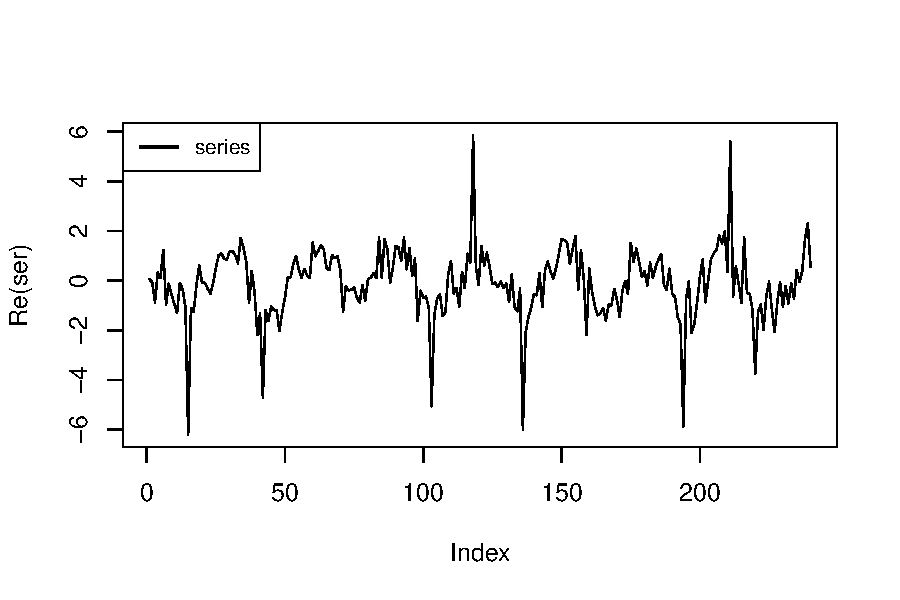
\includegraphics[width=0.67\linewidth]{ser_1_Re.png}
	\end{center}
	\caption{График вещественной части ряда.}
	\label{ser_Re_1}
\end{figure}

\begin{figure}[H]
	\begin{center}
		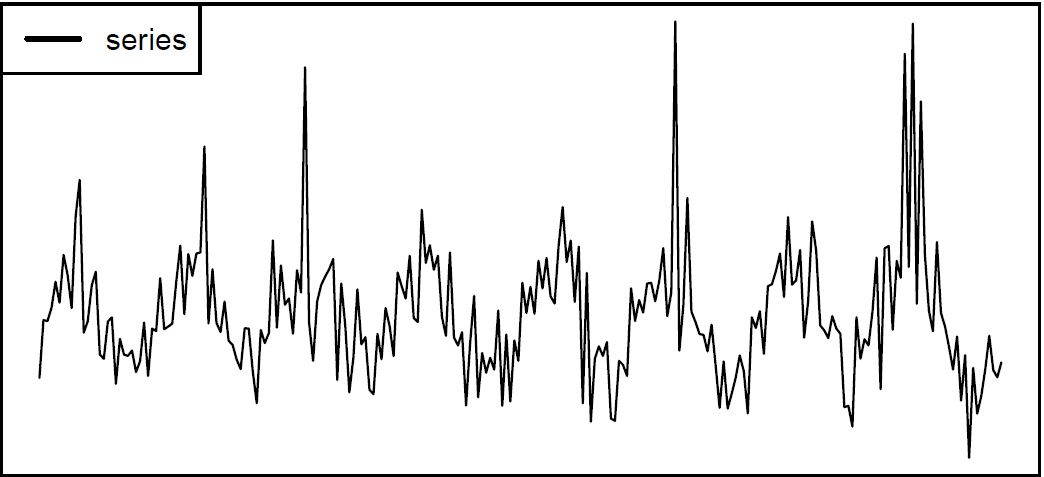
\includegraphics[width=0.67\linewidth]{ser_1_Im.png}
	\end{center}
	\caption{График мнимой части ряда.}
	\label{ser_Im_1}
\end{figure}

Графики результатов анализа представлены в Рис. \ref{analys_Re_1}, \ref{analys_Im_1}. В таблице \ref{tab2} представлены сравнения ошибок для различных методов.  В таблице \ref{tab: pval2} представлены p-value для сравнения методов с лучшим. Длина окна взята $L = 120$.

\begin{figure}[H]
	\begin{center}
		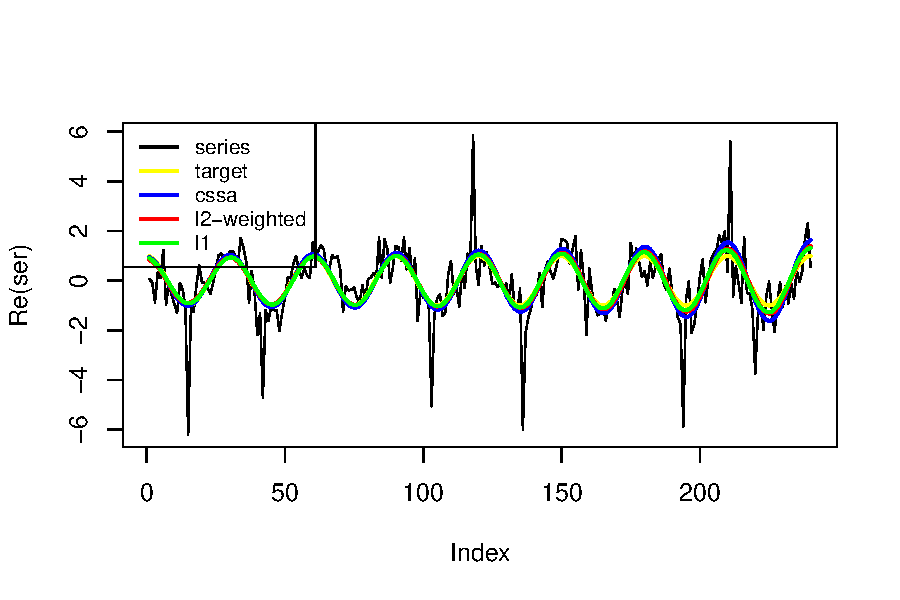
\includegraphics[width=0.67\linewidth]{analys_1_Re.png}
	\end{center}
	\caption{Вещественная часть выделения тренда несколькими способами.}
	\label{analys_Re_1}
\end{figure}

\begin{figure}[H]
	\begin{center}
		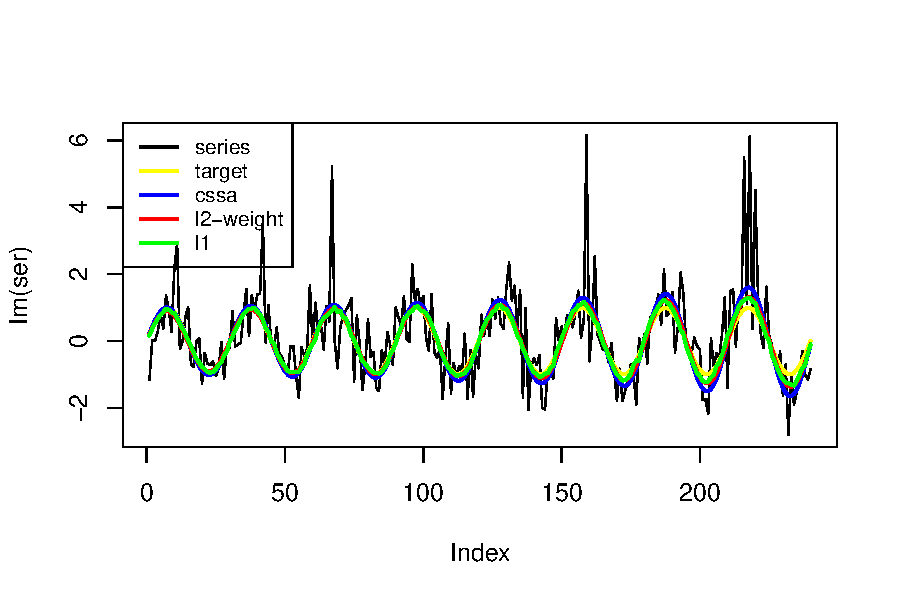
\includegraphics[width=0.67\linewidth]{analys_1_Im.png}
	\end{center}
	\caption{Мнимая часть выделения тренда несколькими способами.}
	\label{analys_Im_1}
\end{figure}

\begin{table}[H]
	\begin{center}
		\caption{Оценки RMSE различных методов для $M = 30$ реализаций ряда с выбросами.}
		\label{tab2}
		\begin{tabular}{|c|c|c|c|c|c|c|}
			\hline
			Method 	& CSSA & L1 & weighted L2 & loess L2 & median L2 & lowess L2 \\ 
			\hline
			RMSE & 0.285  & 0.147  & 0.158 & $\mathbf{0.112}$ & 0.114 & 0.114\\
			\hline
		\end{tabular}
	\end{center}
\end{table}

\begin{table}[H]
	\caption{p-value для сравнения различных методов с наилучшим с выбросами.}
	\label{tab: pval2}
	\begin{center}
		\begin{tabular}{|c|c|c|c|c|c|}
			\hline
			Method & CSSA	& L1 & weighted L2 & median L2 & lowess L2  \\ 
			\hline
			loess L2 & 0  & 7.7e-13 &   4.1e-10  &  \textbf{0.134} & \textbf{0.262}  \\
			\hline
		\end{tabular} \\
	\end{center}
\end{table}

В случае наличия выбросов метод loess проекции на $\mathbb{L}_2$ показал наилучший результат, за исключением того, что сравнения с другими вариациями модифицированной взвешенной проекции незначимы.


\section{Синтетический пример №2}

Рассмотрим ряд с растущей амплитудой и шумом непостоянной дисперсии.
Длину ряда возьмём $N = 240$
$$x_n = e^{4n/N} e^{2n\pi/30i} + \frac{1}{2}e^{4n/N} \varepsilon_n, ~ \varepsilon_n \sim CN(0,1).$$ 
Рассмотрим результаты работы методов для такого ряда (\ref{tab3}).  В таблице \ref{tab: pval3} представлены p-value для сравнения методов с лучшим. Ранг ряда равен 1.

\begin{table}[H]
	\begin{center}
		\caption{Оценки RMSE различных методов для $M = 30$ реализаций ряда без выбросов.}
		\label{tab3}
		\begin{tabular}{|c|c|c|c|c|c|c|}
			\hline
			Method 	& CSSA & L1 & weighted L2 & loess L2 & median L2 & lowess L2 \\ 
			\hline
			RMSE & $\mathbf{1.28}$  & 1.52  & 1.90 & 1.36 & 1.43 & 1.37\\
			\hline
		\end{tabular}
	\end{center}
\end{table}

\begin{table}[H]
	\caption{p-value для сравнения различных методов с наилучшим без выбросов.}
	\label{tab: pval3}
	\begin{center}
		\begin{tabular}{|c|c|c|c|c|c|}
			\hline
			Method & L1 & weighted L2 & loess L2 & median L2 & lowess L2  \\ 
			\hline
			CSSA & 0.005   & 0.0001 & 0.001  & 7.6e-5 & 0.0007  \\
			\hline
		\end{tabular} \\
	\end{center}
\end{table}

В случае отсутствия выбросов лучший результат показывает Complex SSA. Здесь же видно, что модифицированный метод взвешенной проекции справляется с не стационарным рядом куда лучше чем классический, к примеру, сравнивая классический и loess, сравнение является значимым с p-value $ = 0.0005$. 

Теперь добавим к ряду $5\%$ выбросов с величиной выброса $5x_i$. Графики ряда представлены на Рис. \ref{ser_Re_2}, \ref{ser_Im_2}.

\begin{figure}[H]
	\begin{center}
		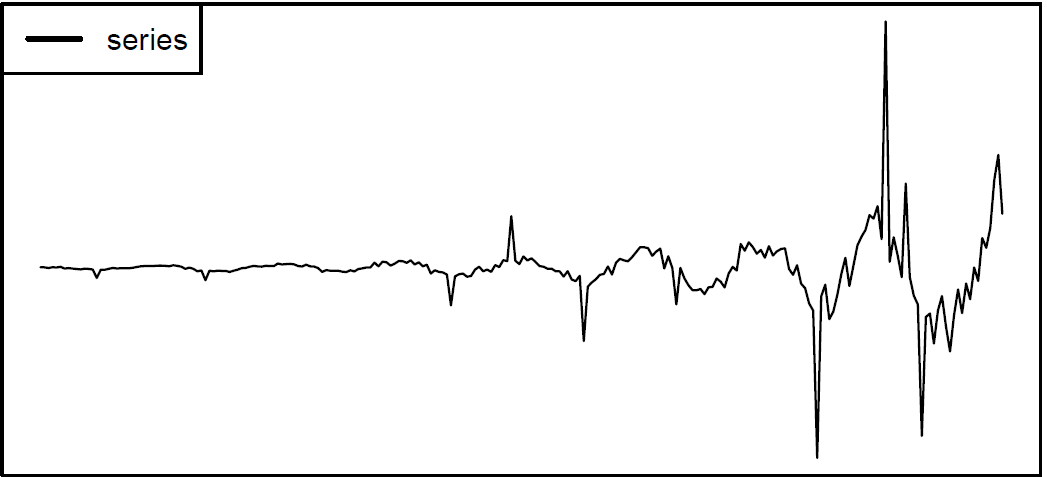
\includegraphics[width=0.67\linewidth]{ser_2_Re.png}
		\caption{График вещественной части ряда.}
		\label{ser_Re_2}
	\end{center}
\end{figure}

\begin{figure}[H]
	\begin{center}
		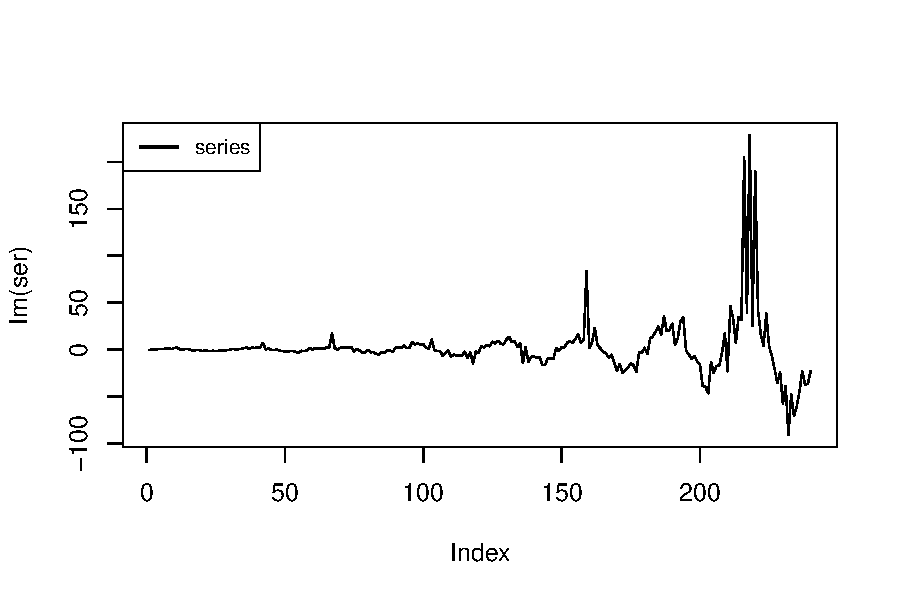
\includegraphics[width=0.67\linewidth]{ser_2_Im.png}
		\caption{График мнимой части ряда.}
		\label{ser_Im_2}
	\end{center}
\end{figure}

Графики результатов анализа представлены на Рис. \ref{analys_Re_2}, \ref{analys_Im_2}. В таблице \ref{tab4} представлены сравнения ошибок для различных методов. В таблице \ref{tab: pval4} представлены p-value для сравнения методов с лучшим. Длина окна взята $L = 120$.

\begin{figure}[H]
	\begin{center}
		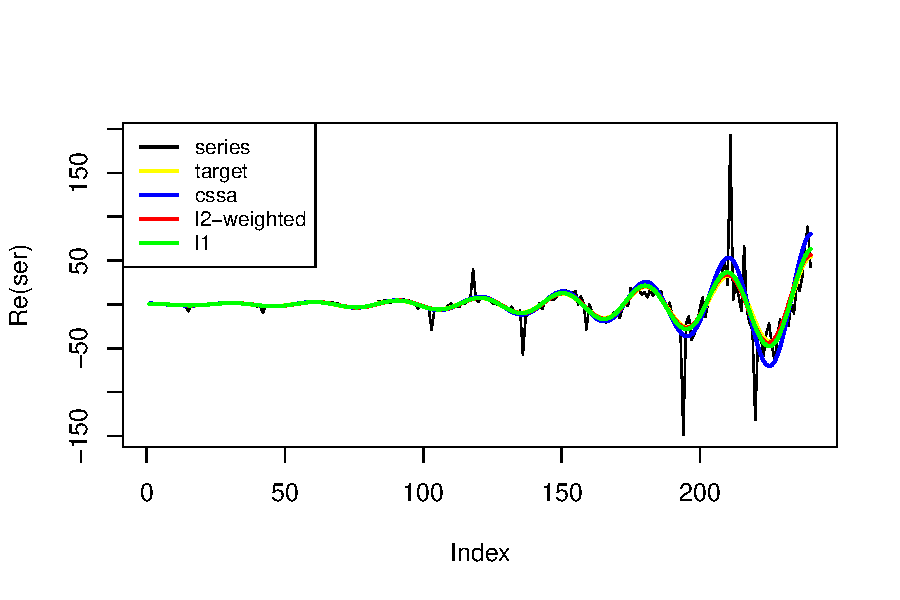
\includegraphics[width=0.67\linewidth]{analys_2_Re.png}
		\caption{Вещественная часть выделения тренда несколькими способами.}
		\label{analys_Re_2}
	\end{center}
\end{figure}

\begin{figure}[H]
	\begin{center}
		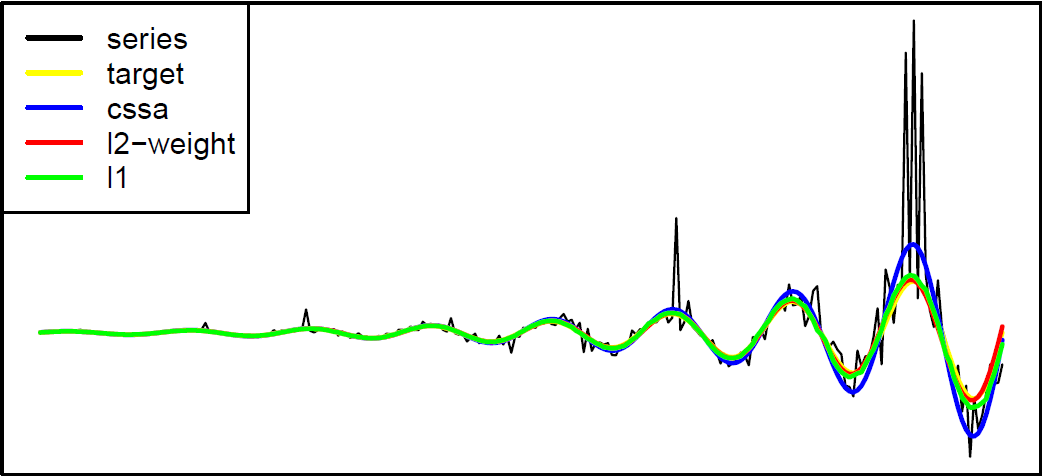
\includegraphics[width=0.67\linewidth]{analys_2_Im.png}
		\caption{Мнимая часть выделения тренда несколькими способами.}
		\label{analys_Im_2}
	\end{center}
\end{figure}

\begin{table}[H]
	\begin{center}
		\caption{Оценки RMSE различных методов для $M = 30$ реализаций ряда с выбросами.}
		\label{tab4}
		\begin{tabular}{|c|c|c|c|c|c|c|}
			\hline
			Method 	& CSSA & L1 & weighted L2 & loess L2 & median L2 & lowess L2 \\ 
			\hline
			RMSE & 6.14  & 1.78  & 1.66 & $\mathbf{1.48}$ & 1.50 & 1.49\\
			\hline
		\end{tabular}
	\end{center}
\end{table}

\begin{table}[H]
	\caption{p-value для сравнения различных методов с наилучшим с выбросами.}
	\label{tab: pval4}
	\begin{center}
		\begin{tabular}{|c|c|c|c|c|c|}
			\hline
			Method & CSSA	& L1 & weighted L2 & median L2 & lowess L2  \\ 
			\hline
			loess L2 & 3.5e-16   & 0.005 &   \textbf{0.13}  &  \textbf{0.387} & \textbf{0.28}  \\
			\hline
		\end{tabular} \\
	\end{center}
\end{table}

В случае присутствия выбросов метод loess проекции на $\mathbb{L}_2$ показывает себя наилучшим образом на данном примере, однако сравнения с взвешенным $\mathbb{L}_2$, median~\ $\mathbb{L}_2$ и lowess $\mathbb{L}_2$ не являются значимыми.



\chapter{Ошибка восстановления}
%\begin{def*}
%	$L$-рангом ряда называется ранг соответствующей ему $L$-траекторной матрицы.
%\end{def*}

Наблюдаем комплексный временной ряд $F$ длины $N$ и длиной окна $L$, данный ряд представляется как $F = S + R$, где $S$~--- сигнал с траекторной матрицей $\mathbf{H} = \mathcal{T}(S)$, $R$~--- возмущение.

В работе \cite{Nekr2008} вводится разложение восстановления сигнала в модели $S(\delta) = S + \delta R$, что соответствует $\mathbf{H}(\delta) = \mathbf{H} + \delta \mathbf{E}$, где $\mathbf{H}(\delta)$~--- траекторная матрица $S(\delta)$, $\mathbf{H}$~--- траекторная матрица $S$, $\delta\mathbf{E}$~--- траекторная матрица возмущения $\delta R$ и рассматривается линейный по $\delta$ член ошибки восстановления, называемый первым. 

Рассмотрим возмущение ряда $R$ с $\delta = 1$ и его траекторная матрица $\mathbf{E}$. Первый член ошибки восстановления обозначим как $f^{(1)} = \mathcal{H}(\mathbf{H}^{(1)})$. 

В \cite{Nekr2008} были получены формулы для $\mathbf{H}^{(1)}$ для вещественных рядов рангов $1$ и $2$. Ниже приведём их комплексное обобщение.

Для $\rk S = 2$ и сингулярных векторов $U_1$, $U_2$, $V_1$, $V_2$ матрицы $\mathbf{H} \mathbf{H}^{\mathrm{H}}$

\begin{multline}\label{eq:main}
\mathbf{H}^{(1)}(\mathbf{E}, S) = U_1 U^{\mathrm{H}}_1 \mathbf{E} + U_2 U^{\mathrm{H}}_2 \mathbf{E} + \mathbf{E} V_1 V^{\mathrm{H}}_1 + \mathbf{E} V_2 V^{\mathrm{H}}_2 -
 \\
 -(\alpha_{11} U_1 V^{\mathrm{H}}_1 + \alpha_{12} U_1 V^{\mathrm{H}}_2 + \alpha_{21} U_2 V^{\mathrm{H}}_1 + \alpha_{22} U_2 V^{\mathrm{H}}_2)
\end{multline}
где $\alpha_{ij} = U_i \mathbf{E} V^{\mathrm{H}}_j$.

Для $\rk S = 1$ и сингулярных векторов $U_1$, $V_1$ 

\begin{equation} \label{eq:main1}
	\mathbf{H}^{(1)}(\mathbf{E}, S) = -U_1^{\mathrm{H}} \mathbf{E} V_1 U_1 V^{\mathrm{H}}_1 + U_1 U^{\mathrm{H}}_1 \mathbf{E} + \mathbf{E} V_1 V^{\mathrm{H}}_1
\end{equation}

Применительно к рассматриваемым методам, приведённые формулы ищут первый член ошибки восстановления для CSSA, тогда как их вещественные аналоги ищут то же для SSA.

Обозначим за:

$f^{(1)} = \mathcal{H}(\mathbf{H}^{(1)}(\mathbf{E}, S))$ первый член ошибки восстановления $S$ метода CSSA,

%$f^{(1)}_{\Re} = \mathcal{H}(\mathbf{H}^{(1)}(\mathbf{\Re(E)}))$ первый член ошибки восстановления $\Re(S)$ метода CSSA,
%
%$f^{(1)}_{\Im} = \mathcal{H}(\mathbf{H}^{(1)}(\mathbf{\Im(E)}))$ первый член ошибки восстановления $\Im(S)$ метода CSSA,

$f^{(1)*}_{\Re} = \mathcal{H}(\mathbf{H}^{(1)}(\mathbf{\Re(E)}, \Re(S)))$ первый член ошибки восстановления $\Re(S)$ метода SSA,

$f^{(1)*}_{\Im} = \mathcal{H}(\mathbf{H}^{(1)}(\mathbf{\Im(E)}, \Im(S)))$ первый член ошибки восстановления $\Im(S)$ метода SSA.

\begin{theorem}\label{th:sum}
	Пусть сингулярные вектора $S$, $\Re(S)$ и $\Im(S)$ совпадают и $\rk S \leq 2$.
	
	Тогда $$f^{(1)} = f^{(1)*}_{\Re(S)} + if^{(1)*}_{\Im(S)}.$$
\end{theorem}
\begin{proof}
	Рассмотрим матрицу возмущения $\mathbf{E} = \Re(\mathbf{E}) + i\Im(\mathbf{E}).$
	
	Заметим, что в \eqref{eq:main} $\mathbf{E}$ входит линейно, это означает, что
	\begin{equation} \label{eq_reim}
		\mathbf{H}^{(1)}(\mathbf{E}, S) = \mathbf{H}^{(1)}(\Re(\mathbf{E}), S) + i\mathbf{H}^{(1)}(\Im(\mathbf{E}), S).
	\end{equation}
%	Совпадение траекторных пространств означает, что правые сингулярные вектора и левые сингулярные вектора $\Re(S)$, $\Im(S)$, добавленное к этому равенство рангов означает, что сингулярные вектора $\Re(S)$, $\Im(S)$ и $S$ совпадают.
%	
	Тогда, из \eqref{eq_reim}, линейности диагонального усреднения и равенства сингулярных векторов, получаем
	\begin{multline*}
		f^{(1)} = \mathcal{H}(\mathbf{H}^{(1)}(\mathbf{E}, S)) = \mathcal{H}(\mathbf{H}^{(1)}(\Re(\mathbf{E}), S)) + i\mathcal{H}(\mathbf{H}^{(1)}(\Im(\mathbf{E}), S)) =\\
		\mathcal{H}(\mathbf{H}^{(1)}(\Re(\mathbf{E}), \Re(S))) + i\mathcal{H}(\mathbf{H}^{(1)}(\Im(\mathbf{E}), \Im(S))) = f^{(1)*}_{\Re} + if^{(1)*}_{\Im}	
	\end{multline*}
	
\end{proof}

\begin{notice*}
	В случае $\rk S = 1$, достаточно требовать совпадающие траекторные пространства вещественной и мнимой части размерности $1$. 
\end{notice*}

\begin{notice*}
	В случае $\rk S = 2$ условию удовлетворяет сигнал $S$ с $\Re(S)~=~\Im(S)$. 
\end{notice*}

%\begin{notice*}
%	Требования теоремы означают существование вещественного базиса в пространстве столбцов $\mathbf{H}$$\mathbf{H}^{\mathrm{H}}$.
%\end{notice*}

\begin{notice*}
	Примером сигнала, для которого в общем случае очевидно не выполняются требования теоремы, является комплексная экспонента $s_n = e^{\phi(n) + i\psi(n)}$, поскольку $\rk S = 1$, а $\rk\Re(S) = \rk\Im(S) = 2$.
\end{notice*}


\section{Шум}

Рассмотрим случай, когда сигнал возмущён шумом $R$ с независимыми вещественной и мнимой частями.

Тогда $\mathbf{E}$~--- траекторная матрица шума $R$.


\begin{notice*}
	Из независимости вещественной и мнимой частей шума и теоремы \ref{th:sum}, $f^{(1)*}_{\Re(S)}$ и $f^{(1)*}_{\Im(S)}$ независимы между собой, как две линейные комбинации независимых наборов.
\end{notice*}

\begin{lemma} \label{std:disp}
	Дисперсия комплексной случайной величины равна сумме дисперсий вещественной и мнимой частей данной случайной величины, если они независимы.
\end{lemma}
\begin{proof}
	$z = x + iy$~--- с.в., 
	\begin{multline*}
		\mathbb{D}z = \mathbb{E}(|z - \mathbb{E}z|^2) = \mathbb{E}(|(x - \mathbb{E}x) + i((y - \mathbb{E}y))|^2) = \\
		= \mathbb{E}(x - \mathbb{E}x)^2 + \mathbb{E}(y - \mathbb{E}y)^2 = \mathbb{D}x + \mathbb{D}y
	\end{multline*}
\end{proof}

\begin{statement} \label{st:dispsum}
	Пусть выполнены условия теоремы \ref{th:sum}.
	
	Тогда
	\begin{equation} \label{eq:dispsum}
	\mathbb{D}f^{(1)}_l = \mathbb{D}f^{(1)*}_{\Re, l} + \mathbb{D}f^{(1)*}_{\Im, l}.	
	\end{equation}
\end{statement}
\begin{proof}
	Получается автоматически из теоремы \ref{th:sum} и леммы \ref{std:disp}.
\end{proof}

\begin{notice*}
	В случае $\rk S = 2$  численными экспериментами, приведёнными в \cite[раздел 4.3.3.3]{Golyandina.etal2018} показано, что равенство \eqref{eq:dispsum} приближённо выполнено для синусоидальных сигналов со сдвигом, не равным $\pi / 2$.
\end{notice*}

\subsection{Частный случай}
Рассматриваем ряд с $s_n = c_1 + ic_2$ и матрицу шума $\mathbf{E}$ с дисперсиями вещественной и мнимой частей $\sigma_1$ и $\sigma_2$.\\
Сингулярные вектора такого ряда являются нормированными векторами с одинаковыми компонентами, они также сингулярные для вещественной и мнимой части. Тогда выполняются условия теоремы \ref{th:sum} и

$$f^{(1)} = f^{(1)*}_{\Re(S)} + if^{(1)*}_{\Im(S)}.$$

В данном случае $\Re(S)$ и $\Im(S)$ являются вещественными константами.

В работе \cite{Vlas2008} была получена аналитическая формула для дисперсии каждого элемента вещественных констант, в нашем случае $f^{(1)*}_{\Re}$ и $f^{(1)*}_{\Im}$.

Обозначим $L = \alpha N$, $\alpha \leq \frac{1}{2}$, $\lambda = \lim_{N\to\infty} 2 l / N$, воспользовавшись утверждением \ref{st:dispsum}, получаем

$$    
\mathbb{D} f^{(1)}_l = \mathbb{D} f^{(1)*}_{\Re, l} + \mathbb{D} f^{(1)*}_{\Im, l} \sim \frac{\sigma^2_1 + \sigma^2_2}{N}
\begin{cases}
	D_1(\alpha, \lambda), &\text{$0 \leq \lambda \leq 2 (1 - 2\alpha)$}\\
	D_2(\alpha, \lambda), &\text{$2 (1 - 2\alpha) < \lambda < 2\alpha$}\\
	D_3(\alpha, \lambda), &\text{$2\alpha \leq \lambda \leq 1$}
\end{cases},
$$
где
\begin{gather*}
	D_1(\alpha, \lambda) = \frac{1}{12 \alpha^2(1 - \alpha)^2} (\lambda^2(\alpha + 1) - 2\lambda\alpha(1 + \alpha)^2 + 4 \alpha(-3\alpha + 3 + 2\alpha^2))\\
	D_3(\alpha, \lambda) = \frac{1}{6 \alpha^2\lambda^2 (\alpha - 1)} (\lambda^4 + 2\lambda^3(3\alpha -2 -3\alpha^2) + \\
	+ 2\lambda^2(3 - 9\alpha + 12\alpha^2 - 4\alpha^3) + 4\lambda(4 \alpha^4 - 4\alpha^3 - 3\alpha^2 + 4\alpha - 1) +\\
	+ 8\alpha - 56 \alpha^2 + 144\alpha^3 - 160\alpha^4 + 64\alpha^5\\
	D_3(\alpha, \lambda) = \frac{2}{3\alpha}.\\
\end{gather*}

Формулы выписаны только до середины ряда из симметричности дисперсии первого порядка ошибки относительно середины ряда.

\section{Выброс}
Рассматриваем временной ряд с константным комплексным сигналом и выбросом $a + ib$, добавленным к $k$-ому элементу сигнала. Матрицу возмущения для выброса $a + ib$ можно записать как  $\mathbf{E} = a\mathbf{G} + ib\mathbf{G}$, где $\frac{1}{a}\Re\mathbf{E} = \frac{1}{b}\Im\mathbf{E}  = \mathbf{G}$. Из теоремы \ref{th:sum} получаем, что достаточно найти вид ошибки для вещественного выброса, общий случай будет выглядеть как эта ошибка для выброса $a$ в вещественной части и эта же ошибка для выброса $b$ в мнимой.  

Рассмотрим временной ряд с константным комплексным сигналом и выбросом $a$, добавленным к $k$-ому элементу сигнала.

Матрица возмущения для выброса $a$
$$\mathbf{E}^{\mathrm{T}} = \begin{pmatrix}
	0 & 0 & 0 & \ldots &  a  & \ldots & 0\\
	 \vdots &\vdots & \vdots & &  \vdots & & \vdots\\
	0 & 0 & a & \ldots & 0 & \ldots & 0\\
	0 & a & 0 & \ldots & 0 & \ldots & 0\\
	a & 0 & 0 & \ldots & 0 & \ldots & 0\\
	\vdots &\vdots & \vdots & & \vdots & & \vdots\\
	0 & 0 & 0 & \ldots & 0 & \ldots & 0\\
\end{pmatrix} \in \mathbb{C}^{K \times L}.$$

$U_1 = \{1/\sqrt{L}\}^{L}_{i = 1},\, V_1 = \{1/\sqrt{K}\}^{K}_{i = 1}$, $K = N - L + 1$, 

Не умаляя общности, будем считать, что $L \leq K$.

\subsection{$0 < k < L$}

Рассматриваем формулу \eqref{eq:main1}
$$\mathbf{H}^{(1)}(\mathbf{E}, S) = -U_1^{\mathrm{H}} \mathbf{E} V_1 U_1 V^{\mathrm{H}}_1 + U_1 U^{\mathrm{H}}_1 \mathbf{E} + \mathbf{E} V_1 V^{\mathrm{H}}_1$$

Рассмотрим члены суммы покомпонентно.

Часть первого слагаемого
$$U_1^{\mathrm{H}} \mathbf{E} = \begin{pmatrix}
	 a/\sqrt{L} & \ldots & a/\sqrt{L} & 0 & \ldots & 0\\
\end{pmatrix}$$

Часть первого слагаемого
$$U_1^{\mathrm{H}} \mathbf{E} V_1 = k a / \sqrt{LK}$$

Часть первого слагаемого
$$U_1 V_1^{\mathrm{H}} = \begin{pmatrix}
	1/\sqrt{LK} & \ldots & 1/\sqrt{LK}\\
	\vdots & & \vdots\\
	1/\sqrt{LK} &   \ldots &  1/\sqrt{LK}
\end{pmatrix}\in \mathbb{C}^{L \times K}
$$
Теперь первое слагаемое целиком
$$U_1^{\mathrm{H}} \mathbf{E} V_1 U_1 V_1^{\mathrm{H}} = \begin{pmatrix}
	k a/ LK & \ldots &  k a/ LK\\
	\vdots & & \vdots\\
	k a/ LK &   \ldots &  k a/ LK
\end{pmatrix}$$

Часть второго слагаемого
$$U_1 U_1^{\mathrm{H}} = \begin{pmatrix}
	1/L & \ldots & 1/L\\
	
	\vdots & & \vdots\\
	1/L &   \ldots &  1/L
\end{pmatrix}\in \mathbb{C}^{L \times L}$$

Теперь второе слагаемое целиком
$$U_1 U_1^{\mathrm{H}} \mathbf{E} = \begin{pmatrix}
	a/L & \ldots & a/L & \ldots & 0\\
	\vdots & & \vdots & & \vdots\\
	a/L & \ldots & a/L & \ldots & 0
\end{pmatrix}$$

Часть третьего слагаемого
$$V_1 V_1^{\mathrm{H}} = \begin{pmatrix}
	1/K & \ldots & 1/K\\
	\vdots & & \vdots\\
	1/K &   \ldots &  1/K
\end{pmatrix}\in \mathbb{C}^{K \times K}$$

Теперь третье слагаемое целиком
$$\mathbf{E} V_1 V_1^{\mathrm{H}} = \begin{pmatrix}
	a/K &  \ldots & a/K\\
	\vdots & & \vdots\\
	a/K &  \ldots & a/K\\
	\vdots & & \vdots\\
	0 & \ldots & 0
\end{pmatrix}$$
Итоговая матрица
$$\mathbf{H}^{(1)} = \frac{a}{LK}\begin{pmatrix}
	(L + K - k) & \ldots & (L + K - k) & \ldots & (L - k)\\
	\vdots & & \vdots & & \vdots \\
	(L + K - k) & \ldots & (L + K - k) & \ldots & (L - k) & \\
	\vdots & & \vdots & & \vdots \\
	(K - k) & \ldots & (K - k) & \ldots & -k \\
\end{pmatrix}$$

$$f^{(1)} = \mathcal{H}(\mathbf{H}^{(1)})$$

$k \leq L/2$

$k \leq K - L$

$$f^{(1)}_l = \frac{a}{{LK}}
\begin{cases}
	(L + K - k), & \text{$1 \leq l \leq k$}\\
	\frac{1}{l}(L + K - l)k, & \text{$k < l \leq L$}\\
	\frac{1}{L}K(L + k - l), &\text{$L < l < L + k$}\\
	0, &\text{$L + k \leq l \leq K$}\\
	\frac{1}{N - l + 1}(K - l)(L - k), &\text{$K < l < K + k$}\\
	-k, &\text{$K + k \leq l \leq N $}
\end{cases}.
$$

$k \leq L/2$

$k > K - L$

$$f^{(1)}_l = \frac{a}{{LK}}
\begin{cases}
	(L + K - k), & \text{$1 \leq l \leq k$}\\
	\frac{1}{l}(L + K - l)k, & \text{$k < l \leq L$}\\
	\frac{1}{L}K(L + k- l), &\text{$L < l < K$}\\
	\frac{1}{N - l + 1}(2KL - l(L + K - k)), &\text{$K \leq l \leq L + k$}\\
	\frac{1}{N - l + 1}( K - l)(L - k), &\text{$L + k < l < K + k$}\\
	-k, &\text{$K + k \leq l \leq N$}
\end{cases}.
$$

$k > L/2$

$k \leq K - L$

$$f^{(1)}_l = \frac{a}{{LK}}
\begin{cases}
	(L + K - k), & \text{$1 \leq l \leq k$}\\
	\frac{1}{l}(L + K - l)k, & \text{$k < l < L$}\\
	%\frac{1}{L}((K + l - 2k)(L - k) + (2k - l)(L + K - k)), & \text{$L\leq l \leq 2k$}\\
	\frac{1}{L}K(L + k - l), &\text{$L \leq l < L + k$}\\
	0, &\text{$L + k \leq l \leq K$}\\
	\frac{1}{N - l + 1}(L - K)(L - k), &\text{$K < l < K + k$}\\
	-k, &\text{$K + k \leq l \leq N$}
\end{cases}.
$$

$k > L / 2$

$k > K - L$

$k \leq K/2$

$$f^{(1)}_l = \frac{a}{{LK}}
\begin{cases}
	(L + K - k), & \text{$1 \leq l \leq k$}\\
	\frac{1}{l}(L + K - l)k, & \text{$k < l < L$}\\
	\frac{1}{L}K(L + k - l), &\text{$L \leq l < K$}\\
	\frac{1}{N - l + 1}(2KL - l(L + K - k)), &\text{$K \leq l \leq L + k$}\\
	\frac{1}{N - l + 1}(L - K)(L - k), &\text{$L + k < l < K + k$}\\
	-k, &\text{$K + k \leq l \leq N$}
\end{cases}.
$$

$k > K/2$


$$f^{(1)}_l = \frac{1}{{LK}}
\begin{cases}
	(L + K - k), & \text{$1 \leq l \leq k$}\\
	\frac{1}{l}(L + K - l)k, & \text{$k < l < L$}\\
	\frac{1}{L}K(L + k - l), &\text{$L \leq l < K$}\\
	\frac{1}{N - l + 1}(2KL - l(L + K - k)), &\text{$K \leq l \leq L + k$}\\
	\frac{1}{N - l + 1}(K - l)(L - k), &\text{$L + k < l < K + k$}\\
	-k, &\text{$K + k \leq l \leq N $}
\end{cases}.
$$

\subsection{$L \leq k \leq K$}

Первое слагаемое
$$U_1^{\mathrm{H}} \mathbf{E} V_1 U_1 V_1^{\mathrm{H}} = \begin{pmatrix}
	a/ K & \ldots &   a/ K\\
	\vdots & & \vdots\\
	a/ K &   \ldots &   a/ K
\end{pmatrix}$$
Второе слагаемое
$$U_1 U_1^{\mathrm{H}} \mathbf{E} = \begin{pmatrix}
	0 & \ldots & a/L & \ldots & a/L & \ldots & 0\\
	\vdots & & \vdots & & \vdots & & \vdots\\
	0 & \ldots & a/L & \ldots & a/L & \ldots & 0
\end{pmatrix}$$
Третье слагаемое
$$\mathbf{E} V_1 V_1^{\mathrm{H}} = \begin{pmatrix}
	a/K &  \ldots & a/K\\
	\vdots & & \vdots\\
	a/K &  \ldots & a/K\\
\end{pmatrix}$$
Итоговая матрица
$$\mathbf{H}^{(1)} = \frac{a}{L}\begin{pmatrix}
	0 & \ldots & 1 & \ldots & 1 & \ldots & 0\\
	\vdots & & \vdots & & \vdots & & \vdots\\
	0 & \ldots & 1 & \ldots & 1 & \ldots & 0
\end{pmatrix}$$

$$f^{(1)}_l = \frac{a}{{L}}
\begin{cases}
	\frac{1}{\min(L, l)}(l - k + L), & \text{$k - L \leq l \leq k$}\\
	\frac{1}{\min(L, N - l + 1)}(L + k - l), & \text{$k < l < L + k$}\\
	0, & \text{иначе}
\end{cases}.$$


\subsection{$K < k \leq N$}
Данный случай полностью аналогичен инвертированному первому случаю, то есть строим ряд для $N - k + 1$ и разворачиваем его.

\vspace{1em}
Полученные формулы были численно проверены для частного случая.

\subsection{Инвариант по RMSE} \label{ss:RMSEinv}

Обозначим $RMSE = \sqrt{\frac{1}{N}\sum_{l = 1}^{N} (f^{(1)}_l)^2}$ для ряда $F = S + R$.

Матрицу возмущения для выброса $a + ib$ можно записать как  $\mathbf{E} = a\mathbf{G} + ib\mathbf{G}$, где $\frac{1}{a}\Re\mathbf{E} = \frac{1}{b}\Im\mathbf{E}  = \mathbf{G}$
\begin{statement}\label{st:RMSEinv}
	Пусть сигнал $S$ удовлетворяет условиям теоремы \ref{th:sum}. 
	
	Тогда RMSE для ряда с сигналом $S$ и выбросом $a + ib$, и  ряда с сигналом $S$ и выбросом $a^* + ib^*$, т.ч. $|a^* + ib^*| = |a + ib|$, совпадают.
\end{statement}
\begin{proof}
	$\mathbf{E} = a\mathbf{G} + ib\mathbf{G}$
	
	По теореме \ref{th:sum} и формулам \eqref{eq:main}, \eqref{eq:main1}
	$$f^{(1)}_l = a\mathcal{H}(\mathbf{H}(\mathbf{G}), \Re(S)) + ib\mathcal{H}(\mathbf{H}(\mathbf{G}), \Im(S)) = c_l(a + bi).$$
	
	Для ряда с сигналом $S$ и выбросом $a + ib$
	$$RMSE = |a + ib|\sqrt{\frac{1}{N}\sum_{l = 1}^{N} c_l^2} $$
	 
	Рассмотрим $a^* + ib^*$, такое что $|a^* + ib^*| = |a + ib|$.
	
	Для ряда с сигналом $S$ и выбросом $a^* + ib^*$
	
	$$RMSE = |a^* + ib^*| \sqrt{\frac{1}{N}\sum_{l = 1}^{N} c_l^2} = |a + ib| \sqrt{\frac{1}{N}\sum_{l = 1}^{N} c_l^2}$$
\end{proof}

\chapter{Ошибки восстановления для комплексной экспоненты}

Наиболее распространенным примером сигнала временных рядов для анализа, является сумма комплексных экспонент. Однако, как замечалось ранее, комплексная экспонента, в общем случае, не удовлетворяет условию теоремы $1$, а потому полученные результаты для такого ряда неприменимы.

В связи с этим, в данном разделе рассматриваются примеры комплексной экспоненты и на них проверяется применимость полученных результатов.  

%\section{Пример}
%При построении комплексных робастных методов возникает вопрос: Что считать выбросом? В данной работе выброс считается как элемент с аномально большим модулем. В связи с этим возникает другой вопрос: Не могут ли возникнуть проблемы в случае несимметричности распределения модуля выброса по вещественной и мнимой части? То есть не может ли получиться такой ситуации, что алгоритм посчитает выбросом точку, имеющую очень большое отклонение по вещественной оси, но на мнимой оси эта точка выбросом не является, что приведёт к ухудшению выделения тренда по мнимой оси.
%
%Для рассмотрения примера на тему возьмём прошлый ряд, но выбросы сосредоточим только на вещественной оси, их вещественную часть оставив прежней. Так же в данном примере будет осмыслено посчитать помимо совместных ошибок ещё и отдельно ошибки вещественной и мнимой частей.
%
%Графики выделения тренда представлены на Рис. \ref{analys_Re_3}, \ref{analys_Im_3}. Результаты RMSE для примера представлены в таблице \ref{tab5}. Так же посчитаем RMSE отдельно для вещественной и мнимой части для прошлого примера, для которого выбросы по модулю сделаем равными текущим, результат в таблице \ref{tab6}.
%%Значения p-value представлены в таблице \ref{tab: pval5}. 
%
%\begin{figure}[H]
%	\begin{center}
%		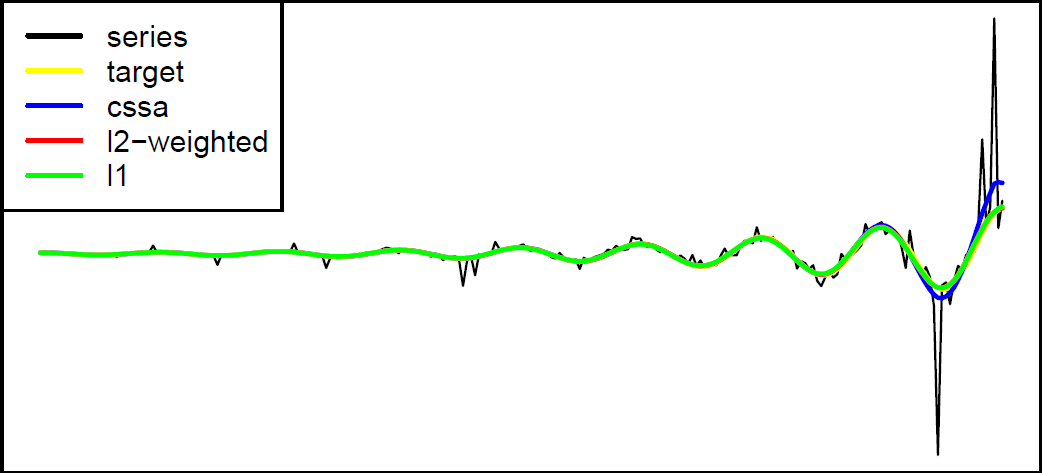
\includegraphics[width=0.67\linewidth]{analys_3_Re.png}
%		\caption{Вещественная часть выделения тренда несколькими способами.}
%		\label{analys_Re_3}
%	\end{center}
%\end{figure}
%
%\begin{figure}[H]
%	\begin{center}
%		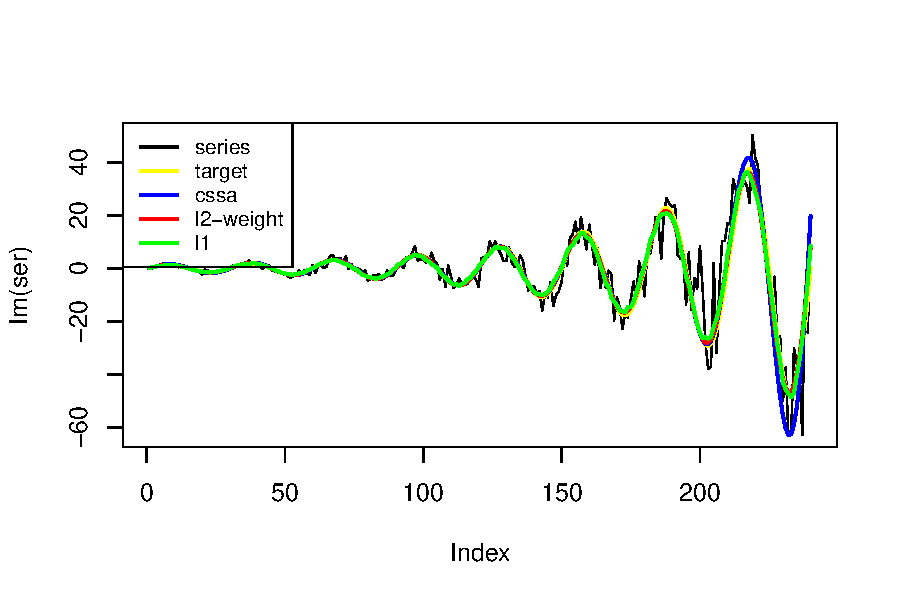
\includegraphics[width=0.67\linewidth]{analys_3_Im.png}
%		\caption{Мнимая часть выделения тренда несколькими способами.}
%		\label{analys_Im_3}
%	\end{center}
%\end{figure}
%
%\begin{table}[H]
%	\begin{center}
%		\caption{Оценки RMSE различных методов для $M = 30$ реализаций ряда с вещественными выбросами.}
%		\label{tab5}
%		\begin{tabular}{|c|c|c|c|c|c|c|}
%			\hline
%			Method 	& CSSA & L1 & weighted L2 & loess L2 & median L2 & lowess L2 \\ 
%			\hline
%			RMSE (совм.) & 3.53  & 1.55  & 1.72 & $\mathbf{1.45}$ & 1.48 & 1.46\\
%			\hline
%			RMSE (Re) & 2.63  & 1.06  & 1.23 & $\mathbf{1.05}$ & 1.07 & 1.06\\
%			\hline
%			RMSE (Im) & 2.33  & 1.14  & 1.2 & $\mathbf{0.98}$ & 1.02 & 1\\
%			\hline
%		\end{tabular}
%	\end{center}
%\end{table}
%
%\begin{table}[H]
%	\begin{center}
%		\caption{Оценки RMSE различных методов для $M = 30$ реализаций прошлого примера.}
%		\label{tab6}
%		\begin{tabular}{|c|c|c|c|c|c|c|}
%			\hline
%			Method 	& CSSA & L1 & weighted L2 & loess L2 & median L2 & lowess L2 \\ 
%			\hline
%			RMSE (совм.) & 3.53  & 1.29  & 1.34 & $\mathbf{0.97}$ & 1 & 0.98\\
%			\hline
%			RMSE (Re) & 2.5  & 0.85  & 0.95 & $\mathbf{0.7}$ & 0.71 & $\mathbf{0.7}$\\
%			\hline
%			RMSE (Im) & 2.5  & 0.97  & 0.95 & $\mathbf{0.69}$ & 0.71 & $\mathbf{0.7}$\\
%			\hline
%		\end{tabular}
%	\end{center}
%\end{table}
%
%%\begin{table}[H]
%%	\caption{p-value для сравнения различных методов с наилучшим с выбросами.}
%%	\label{tab: pval5}
%%	\begin{center}
%%		\begin{tabular}{|c|c|c|c|c|c|}
%%			\hline
%%			Method & CSSA	& L1 & weighted L2 & median L2 & lowess L2  \\ 
%%			\hline
%%			loess L2 (совм.) & 1.1e-08  & \textbf{0.166} &  0.028  & \textbf{0.46} & \textbf{0.756}  \\
%%			\hline
%%			loess L2 (Re) & 1.4e-08  & \textbf{0.69} &  \textbf{0.073}  & \textbf{0.54} & \textbf{0.8}  \\
%%			\hline
%%			loess L2 (Im) & 3e-08  & 0.0014 &  0.001  & \textbf{0.19} & \textbf{0.26}  \\
%%			\hline
%%		\end{tabular} \\
%%	\end{center}
%%\end{table}
%
%Получаем, что общая ошибка в случае, когда выбросы равномерно распределены по вещественной и по мнимой оси ниже, но распределение ошибок по вещественной и мнимой осям сохраняется. Что свидетельствует в пользу нашего предположения и кажется разумным для данных методов, как для методов, приближающих весь комплексный ряд, а не вещественную и мнимую части по отдельности.


\section{Вещественные выбросы}

Рассмотрим случай вещественных выбросов для комплексной экспоненты. Попробуем проверить результат теоремы \ref{th:sum} для этого случая на примере.

Будем рассматривать экспоненту без шума, длины $N = 240$
$$x_n = e^{4n/N} e^{2n\pi/30i}.$$
с $5\%$ выбросов вида $5 \Re(x_i)$.

Графики ряда представлены на Рис. \ref{ser_Re_5}, \ref{ser_Im_5}.

\begin{figure}[H]
	\begin{center}
		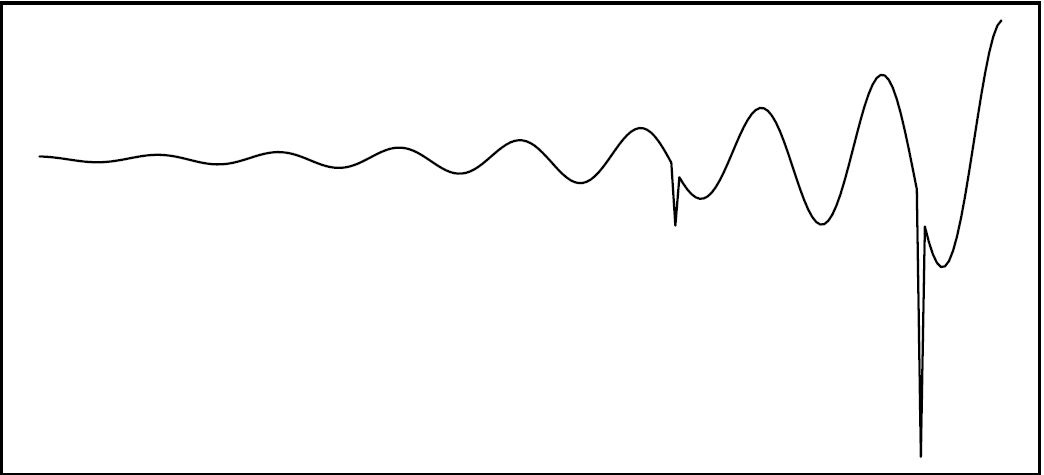
\includegraphics[width=0.67\linewidth]{Re_outl_Re.png}
		\caption{График вещественной части ряда.}
		\label{ser_Re_5}
	\end{center}
\end{figure}

\begin{figure}[H]
	\begin{center}
		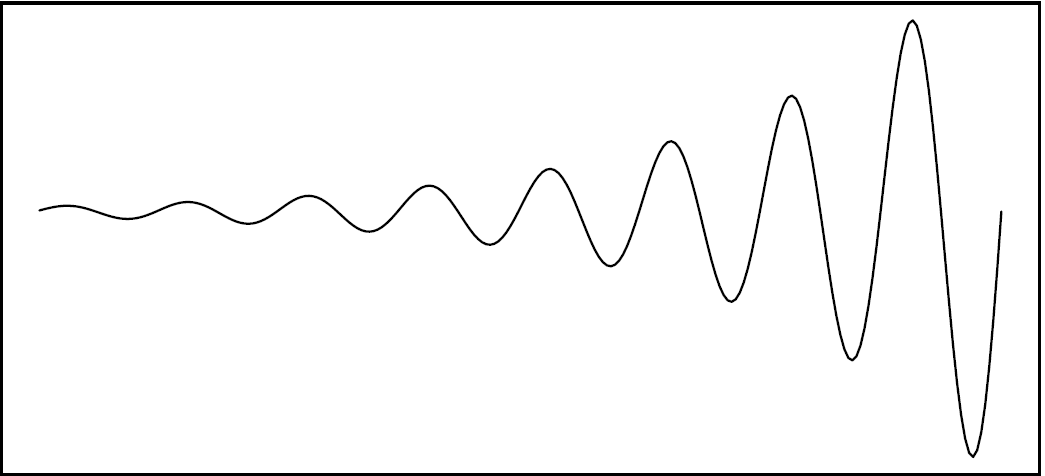
\includegraphics[width=0.67\linewidth]{Re_outl_Im.png}
		\caption{График мнимой части ряда.}
		\label{ser_Im_5}
	\end{center}
\end{figure} 


%\subsection{Модификация функции весов}
%
%У этого ряда все выбросы находятся в вещественной части. Разумно воспользоваться этой информацией и при идентификации выбросов смотреть лишь на вещественную часть, чтобы уменьшить ошибку.
%
%В выбранной нами в данной работе функции весов выброс идентифицируется по модулю числа. Первое, что приходит на ум~--- модифицировать функцию весов, чтобы она реагировала исключительно на вещественную часть. Тогда получаем 
%$$w(x) = 
%\begin{cases}
%	(1 - (\frac{|\Re(x)|}{\alpha})^2)^2 &|\Re(x)| \leq \alpha\\
%	0 &|\Re(x)| > \alpha\\
%\end{cases}.$$
%
%Проведём сравнение ошибок двух алгоритмов, с $|x|$ и $|\Re(x)|$ для предложенного примера. Результаты в таблице \ref{tab7}, ошибки приведены отдельно для всего ряда, вещественной и мнимой частей.
%
%\begin{table}[H]
%	\begin{center}
%		\caption{сравнения RMSE}
%		\label{tab7}
%		\begin{tabular}{|c|c|c|c|}
%			\hline
%			Ряд & w-L2 abs & w-L2 Re & p-value \\ 
%			\hline
%			complex & 0.053  & 0.053 & 0.62 \\
%			\hline
%			Re & 0.037  & 0.037 & 0.56 \\
%			\hline
%			Im & 0.38  & 0.038 & 0.69 \\
%			\hline
%		\end{tabular}
%	\end{center}
%\end{table}
%
%Получили, что модификация не дала прироста в ошибке даже по вещественной оси.

Для данного ряда рассмотрим $\Re(f^{(1)})$ и $\Im(f^{(1)})$, проверим, ведут ли они себя так же, как $f^{(1)*}_{\Re}$ и $f^{(1)*}_{\Im}$.

Графики $\Re(f^{(1)})$ и $\Im(f^{(1)})$ приведены на Рис. \ref{f1}.

\begin{figure}[H]
	\begin{center}
		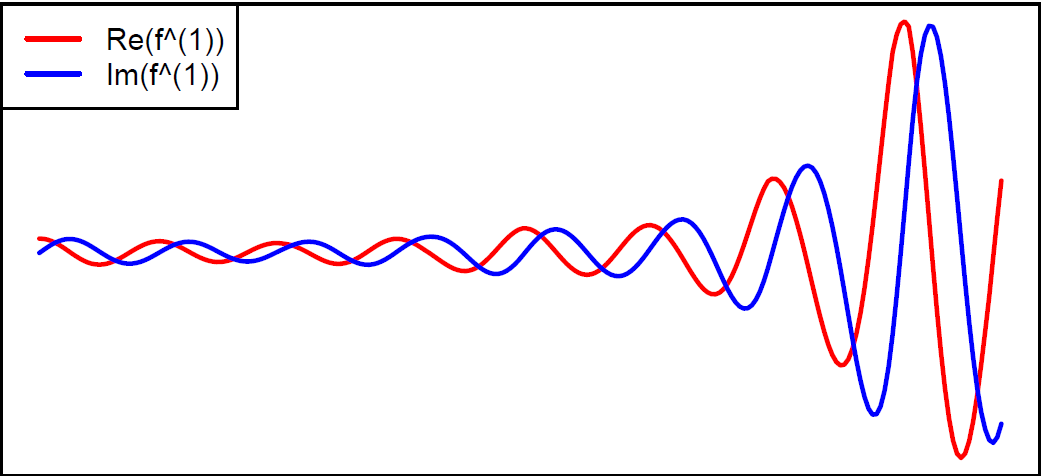
\includegraphics[width=0.67\linewidth]{f1.png}
		\caption{Графики $\Re(f^{(1)})$ и $\Im(f^{(1)})$.}
		\label{f1}
	\end{center}
\end{figure}

По представленным графикам видно, что вещественная и мнимая части ошибки восстановления ведут себя одинаково, тогда как $f^{(1)*}_{\Im} = 0$, а $f^{(1)*}_{\Re} \neq 0$ из-за того, что все выбросы в вещественной части. Получаем, что результат теоремы \ref{th:sum} не выполняется для общего случая комплексной экспоненты.


%\section{Инвариантное по RMSE преобразование}
%
%В разделе \ref{ss:RMSEinv} был найден инвариант по RMSE для рядов, удовлетворяющих теореме \ref{th:sum}.
%
%Проверим, является ли преобразование, сохраняющее модули, инвариантом по RMSE для случая комплексной экспоненты
%
%Рассмотрим ряд с растущей амплитудой и шумом непостоянной дисперсии.
%Длину ряда возьмем $N = 240$
%$$x_n = e^{4n/N} e^{2n\pi/30i} + \frac{1}{2}e^{4n/N} \varepsilon_n, ~ \varepsilon_n \sim CN(0,1).$$
%и $5\%$ выбросов с величиной выброса $4x_i$.
%
%Графики ряда представлены на Рис. \ref{ser_Re_3}, \ref{ser_Im_3}.
%
%\begin{figure}[H]
%	\begin{center}
%		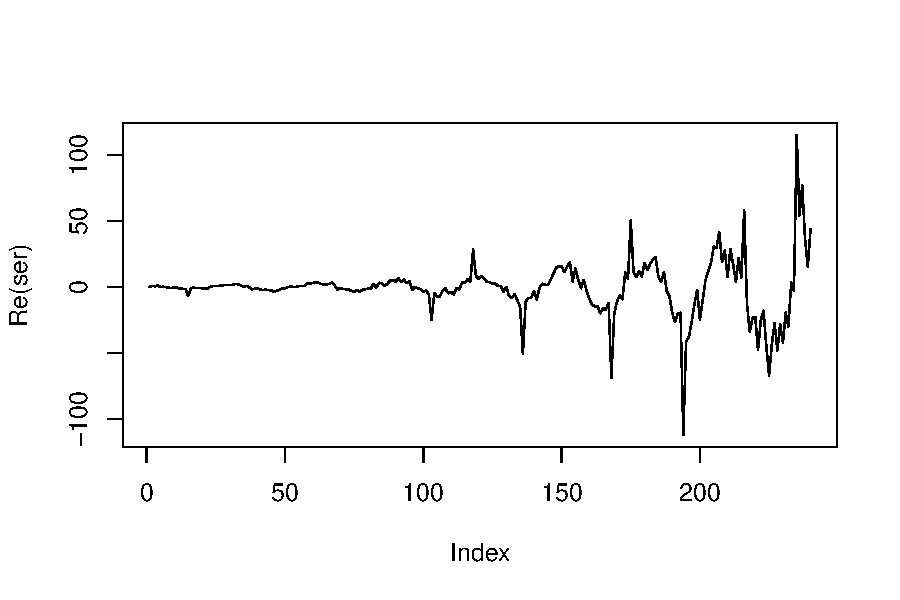
\includegraphics[width=0.67\linewidth]{ser_3_Re.png}
%		\caption{График вещественной части ряда.}
%		\label{ser_Re_3}
%	\end{center}
%\end{figure}
%
%\begin{figure}[H]
%	\begin{center}
%		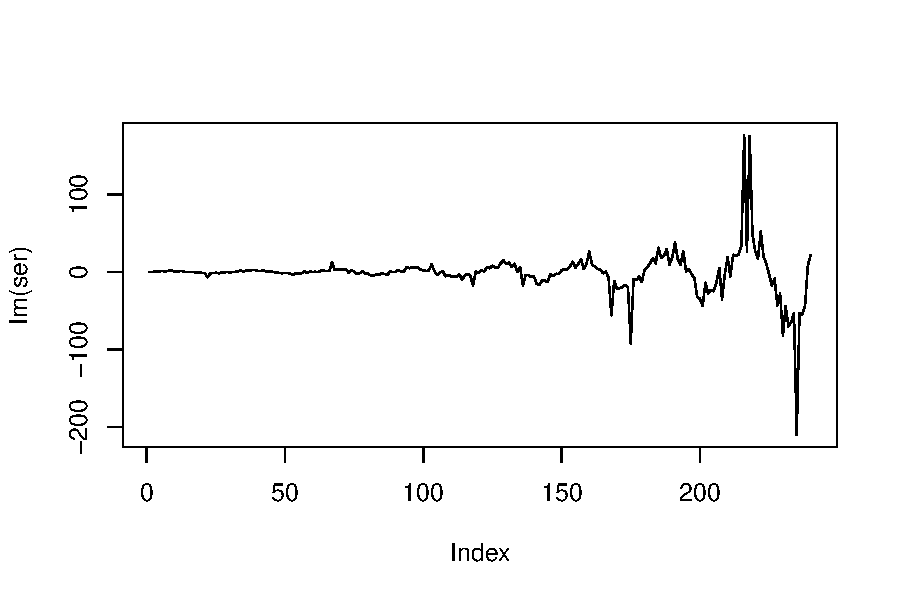
\includegraphics[width=0.67\linewidth]{ser_3_Im.png}
%		\caption{График мнимой части ряда.}
%		\label{ser_Im_3}
%	\end{center}
%\end{figure} 
%
%Теперь поймем, какое преобразование сохраняет модуль, найдем вещественное $c_i$ такое, что\\
%$|x_i + c_i| = |x_i + 4 x_i|$.
%
%Пусть $\Re(x_i) = a_i$, $\Im(x_i) = b_i$, тогда
%$$\sqrt{(c_i + a_i)^2 + b_i^2} = \sqrt{25 a_i^2 + 25 b_i^2}$$
%$$(c_i + a_i)^2 = 25 a_i^2 + 24 b_i^2$$
%$$|c_i| = \sqrt{25 a_i^2 + 24 b_i^2} - a_i$$
%
%Не умаляя общности, можно рассмотреть знак $c_i$, совпадающим с $x_i$.
%Тогда рассмотрим тот же ряд с $5\%$ выбросов, но с величиной выброса $\sign(x_i)(\sqrt{25 \Re(x_i)^2 + 24 \Im(x_i)^2} - \Re(x_i))$.
%
%Графики ряда представлены на Рис. \ref{ser_Re_4}, \ref{ser_Im_4}.
%
%\begin{figure}[H]
%	\begin{center}
%		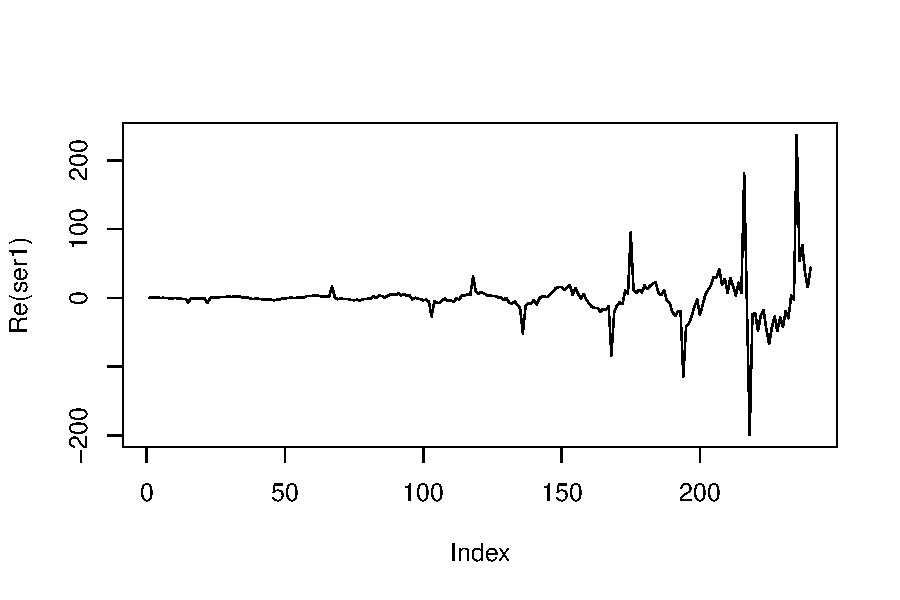
\includegraphics[width=0.67\linewidth]{ser_4_Re.png}
%		\caption{График вещественной части ряда.}
%		\label{ser_Re_4}
%	\end{center}
%\end{figure}
%
%\begin{figure}[H]
%	\begin{center}
%		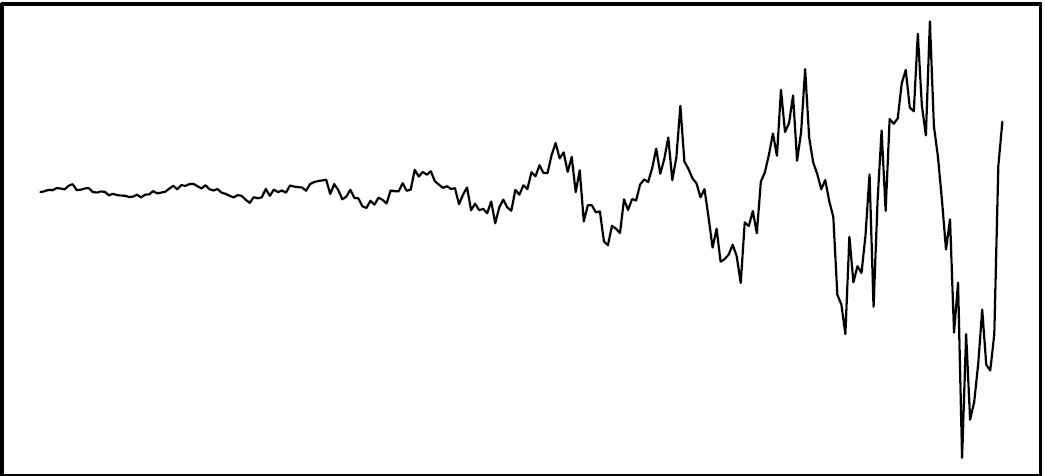
\includegraphics[width=0.67\linewidth]{ser_4_Im.png}
%		\caption{График мнимой части ряда.}
%		\label{ser_Im_4}
%	\end{center}
%\end{figure} 
%
%
%Результаты сравнений RMSE на двух рядах приведены в таблице \ref{pvaltab}.
%
%\begin{table}[H]
%	\begin{center}
%		\caption{p-value сравнения RMSE}
%		\label{pvaltab}
%		\begin{tabular}{|c|c|c|c|c|}
%			\hline
%			Ряд  & CSSA & L1 & w-L2 & mod. w-L2 \\ 
%			\hline
%			complex & 0.0045 & 0.51  & 0.65 & 0.56 \\
%			\hline
%			Re & 0.06 & 0.43 & 0.64 & 0.46 \\
%			\hline
%			Im & 0.0002 &0.57  & 0.66 & 0.72 \\
%			\hline
%		\end{tabular}
%	\end{center}
%\end{table}
%
%Как мы видим, гипотеза о различии RMSE на двух рядах значима для CSSA, особенно для мнимой части, то есть данное преобразование не является инвариантом для CSSA в случае комплексной экспоненты. 
%
%Для остальных методов гипотеза незначима. То есть преобразование, сохраняющее модули, является инвариантом. Можно предположить, что это связано с тем, что в каждом из них выброс идентифицируется по своему модулю.


\newpage
\conclusion
%\section{Заключение}
В работе были приведены и исследованы два обобщения робастных вариантов метода SSA на комплексно-значный случай. 

Был проведён обзор двух известных подходов к построению робастных версий SSA: замена проекции по норме $\mathbb{L}_2$ на проекцию по норме $\mathbb{L}_1$ и на взвешенную проекцию по норме $\mathbb{L}_2$ и их имплементация на комплексный случай.

%В предположении, что число итераций не зависит от длины ряда, было произведено сравнение трудоёмкостей методов. Метод %проекции на $\mathbb{L}_1$ оказался наименее трудоёмким.

Работа методов была показана на нескольких примерах, подтверждающих эффективность робатсных модификаций, в сравнении с Complex SSA для рядов с выбросами. Все рассматриваемые модификации были реализованы на R.

В подотчётном семестре формула первого ошибки восстановления для рядов методом CSSA, ранга не больше двух, была рассмотрена и обобщена на комплексный случай. Была сформулирована и доказана теорема о выражении первого порядка ошибки метода CSSA через ошибку метода SSA.

Был разобран случай возмущения ряда шумом. Для него было сформулировано и доказано утверждение о выражении дисперсии ошибки метода CSSA через ошибку метода SSA. Для случая константного комплексного ряда была получена явная формула дисперсии  первого порядка ошибки восстановления для каждого элемента ряда.

Был разобран случай возмущения ряда единичным выбросом. Для случая константного ряда была получена явная формула первого порядка ошибки восстановления для каждого элемента. Для более общего случая было найдено инвариантное по RMSE преобразование, переводящее комплексный выброс в вещественный, с сохранением RMSE.

Помимо этого был рассмотрен пример комплексной экспоненты, на которую не распространяются полученные теоретические результаты, с вещественными выбросами. Было показано, что теорема о выражении первого порядка ошибки для CSSA через ошибку для SSA неприменима в этом случае. Так же было показано, что найденное преобразование не является инвариантом для CSSA в этом случае, но для остальных методов, на конкретном примере, это инвариант.    

\nocite{*}
\bibliographystyle{ugost2008}
\bibliography{literature}    

\end{document}
